\documentclass[12pt]{article}
\usepackage{amsmath,amssymb}
\usepackage[right=1.25in,left=1.25in,top=1.15in,bottom=1.1in]{geometry}
\usepackage{setspace}
\usepackage{makecell}
\usepackage[backref=page]{hyperref}
\renewcommand*{\backref}[1]{}
\renewcommand*{\backrefalt}[4]{%
	\ifcase #1 (Not cited.)%
	\or        [Cited on page~#2.]%
	\else      [Cited on pages~#2.]%
	\fi}
\usepackage{xcolor}
\definecolor{mLightBrown}{rgb}{0.92,0.51,0.1}
\hypersetup{
    colorlinks,
    linkcolor={mLightBrown},
    citecolor={mLightBrown},
    urlcolor={mLightBrown}
}

\usepackage[longnamesfirst]{natbib}
\usepackage{adjustbox}
\usepackage{threeparttable}
\usepackage{booktabs}
\usepackage{caption}
\usepackage{subcaption}
\usepackage{pdflscape} 
\usepackage{graphicx} 
\usepackage{tikzit}
\usetikzlibrary{positioning}
\usetikzlibrary{calc}
\usetikzlibrary{arrows.meta}
\newcommand*\diff{\mathop{}\!\mathrm{d}}
\usepackage{tikz}

\newcommand{\E}{\mathbb{E}}
\newcommand{\mc}{\mathcal}

\title{{\LARGE Illiquid Homeownership and the \\ Bank of Mom and Dad}\thanks{Federal Reserve Board of Governors. E-mail: eirik.e.brandsaas@frb.gov. I have benefited from the comments of Dean Corbae, Erwan Quintin, Ananth Seshadri, Corina Mommaerts, Corina Boar, Manuel Amador, Hamish Low, Patrick Moran, Dionissi Aliprantis, David Sturrock, Mike Eriksen, Aradhya Sood, Margaret Jacobson, William Gamber, Claudia Sahm, and Joel McMurry, as well as seminar participants Oxford Sa{\"i}d, Federal Reserve Board, Cal State Fullerton, Boston Fed, ECARES/Université libre de Bruxelles, Santa Clara, University of Lugano, NYU Furman, Norges Bank, BI Norwegian Business School, UW-Madison, and conference participants at NASEMS, AREUEA National, ReCapNet, Minneapolis Fed/OIGI, UEA EU, CFPB, CEF, SAET, Oxford NuCamp Macro Workshop, YES 2020 at UPenn, and Minnesota-Wisconsin Macro/International Workshop. Code and replication instructions are available at the \href{https://github.com/eirikbrandsaas/HomeownershipBankMomDad.jl}{author's  website and Github}.\newline \textit{Disclaimer: }The views expressed in this paper are solely the responsibility of the author and should not be interpreted as reflecting the views of the Board of Governors of the Federal Reserve System or of anyone else associated with the Federal Reserve System.}}
\author{Eirik Eylands Brandsaas}
\date{{\today }}

\begin{document}

\maketitle
\begin{abstract}
{\begin{spacing}{1.2}
Housing is the largest asset in U.S. household portfolios, and first-time homebuyers increasingly rely on parental transfers. This paper quantifies the contribution of parental transfers to the homeownership rate of young households. I build and estimate a life-cycle overlapping generations model with housing, where adult children and parents interact without commitment. I find that parental transfers account for 14 percentage points (29\%) of young households' homeownership. Transfers from wealthy parents not only help households overcome borrowing constraints, but also help sustain homeownership, mitigating the drawbacks of illiquidity. Surprisingly, policies lowering entry barriers to homeownership generally increase the reliance on parental wealth, whereas increased liquidity reduces it. Finally, I show that children of wealthy parents strategically use the illiquidity of housing as a commitment device to encourage transfers, resulting in a preference for illiquidity.
\end{spacing}}
\vspace{0.5cm}
\noindent \textbf{JEL:} D14, D15, E21, G51, R21

\noindent \textbf{Keywords:} Homeownership, Parental transfers, Altruism, Life-cycle models

\end{abstract}
\newpage
\onehalfspacing

\section{Introduction}
Housing is the largest asset in U.S. household portfolios. While homeownership is seen as central to the ``American Dream'' \citep{goodman2018homeownership}, households face different barriers to ownership. Between 2009 and 2016, around 30\% of American first-time homebuyers received direct parental assistance for their down payment, with such assistance averaging \$48,000 per receiving household\textcolor{red}{Check numbers}.\footnote{All data from the Survey of Household Economic Decisionmaking and the Panel Study of Income Dynamics (see Section \ref{sec:data}).} This assistance highlights disparities in access, as only those with sufficiently wealthy parents can expect substantial transfers.

This paper quantifies the importance of parental transfers for young adults' homeownership and investigates how policies lowering homeownership barriers interact with parental transfers. A growing literature emphasizes that families matter for economic outcomes \citep{Doepke2016a}. In the context of homeownership, previous empirical studies highlight that parental transfer receipt is associated with an increase in the probability of becoming a homeowner, mainly by relaxing credit constraints \citep[see e.g.,][]{Lee2018,Blickle2019,wold2024housing}. Additionally, parental transfers help households maintain homeownership, a mechanism that has received less attention \citep[see e.g.,][]{bond2021role}. However, while these studies show that transfer receipt increases the probability of renters becoming homeowners, they do not address the overall importance of parental transfers. For example, households may anticipate future transfers and subsequently save less. In this case, even if transfers increase the likelihood of homeownership, all else being equal, they may not affect aggregate homeownership. Furthermore, this is the first paper quantifying the importance of parental transfers as a determinant of homeownership; the existing literature has primarily focused on family formation and credit constraints \citep[see e.g.,][]{Chang2024,Paz-Pardo2019,Mabille2020}.

I first present empirical evidence indicating that parental wealth helps not only in the transition to ownership, but also in maintaining ownership. \textcolor{red}{bring in new empirical results here. Highlight that the results on behind and unemployment are new}. I show that, controlling for a wide set of household and parental characteristics, households with wealthier parents are less likely to fall behind on mortgage payments after becoming homeowners, even though they buy more expensive homes. Finally, using a variation of the event study in \cite{Chetty2007}, I show that while most households downsize their housing during unemployment spells, those with wealthy parents retain their current homes.

To quantify the impact of parental transfers on homeownership, I then combine two distinct models: housing models, which ignore parental transfers, and models of parental transfers, which ignore housing. I build a life-cycle overlapping generations model with altruistic parents and a rent-or-own decision. Parents and children interact without commitment through both inter-vivos transfers and end-of-life bequests. In models of altruism without housing (e.g., \citealp{Altonji1997a,Barczyk2014}), the transfer motive is to increase the child's consumption when they are borrowing constrained, thus having high marginal utility of wealth. The inclusion of a frictional housing market generates two new transfer motives. First, transfers can directly alleviate credit constraints, enabling wealthier parents to help their children meet down-payment requirements. Second, future transfers provide partial insurance against future income shocks, reducing risks associated with the large illiquid investment of homeownership. Moreover, the illiquidity of housing serves as a commitment device enabling children to secure future transfers. These mechanisms differ from those examined by \citet{Barczyk2020a}, who study how elderly parents’ homeownership decisions shape nursing‑home entry, care arrangements, and intergenerational transfers. As in all transfer models, the expectation of future transfers reduces children's saving motives, potentially lowering the homeownership rate.

Allowing for parental transfers in all periods highlights that transfers are critical not only for entering homeownership---the main focus of empirical literature---but also for maintaining homeownership. Specifically, the prospect of future transfers mitigates the downsides of homeownership for liquidity-constrained households. Ameliorating illiquidity turns out to be as important as relaxing borrowing constraints. Crucially, the model rationalizes the previously discussed empirical pattern that households with wealthy parents do not downsize during income losses, which would not be possible without allowing transfers in all periods. 

I estimate the model by matching data on homeownership, wealth, and transfers from the Panel Study of Income Dynamics (PSID). To quantify the importance of transfers, I find the counterfactual homeownership rate without parental transfers. Without parental transfers, the model simplifies to a standard life-cycle model with housing. I find that parental transfers account for 14 percentage points (29\%) of the homeownership rate among young households. 

I then use the model to evaluate policies aiming to increase homeownership. I find that such policies disproportionately benefit households with wealthy parents. Relaxing mortgage constraints---for example, by lowering minimum down payments---strengthens the link between parental wealth and children's housing outcomes, since more households with wealthy parents are on the margin to become homeowners. Nonmortgage policies that lower barriers to entry, such as reducing prices or purchase costs, increase homeownership for all households, though disproportionately among those with wealthier parents. However, increasing liquidity by reducing sales costs weakens the link between parental wealth and children's housing outcomes, as the partial insurance provided by parental wealth becomes less important.

I then study how illiquidity affects the strategic behavior arising in the absence of commitment. I find that 27\% of young households prefer illiquid housing---due to sales costs---to liquid housing. These households have wealthy parents and use the sales costs as a commitment device to maintain low liquid wealth in the next period, effectively becoming ``wealthy hand-to-mouth.'' Lower liquid wealth implies higher marginal propensities to consume (MPC) and, hence, more parental transfers. As an illustrative example, consider a child who buys a house and brings no liquid wealth to the next period. If the parent does not transfer in the next period, the child will either face very low consumption (with a correspondingly high marginal value of wealth) or be forced to liquidate the house and incur sales costs. The parent dislikes both outcomes and may find it optimal to transfer enough to keep the child in the home. This driver of preference for illiquidity differs from those studied in the literature, such as temptation or time inconsistency \citep{attanasio2024temptation,laibson1997golden}. Furthermore, parental wealth generating preference for illiquidity provides a novel explanation for the existence of high-MPC households \cite[see e.g.,][]{kaplan2022marginal}. That children with wealthy parents find illiquidity less problematic---or even prefer it---is consistent with the empirical results in \cite{choukhmane2023benefits}. They find that households with wealthy parents are more likely to invest in illiquid retirement accounts and less likely to make costly early withdrawals, even after controlling for a wide set of characteristics. 

Finally, I quantify the contribution of parental transfers to the Black-White homeownership gap of 50\% among young adults. I adapt the methodology of \cite{Ashman2020} and \cite{aliprantis2022dynamics}, who study the racial wealth gap, and recalibrate the income process to capture racial differences. I find that parental transfers account for 7 percentage points (14\%) of the Black-White homeownership gap. For context, the Black-White homeownership gap has remained roughly constant since the passing of the Fair Housing Act in 1968.



%%%%%
%% Start of pure literature review
%%%%%

My paper first contributes to the literature studying the determinants of homeownership over the life cycle. Recent papers focus on marriage and family formation \citep{Fisher2011,Chang2024,Khorunzhina2019}, housing demand in old age \citep{McGee2019,Barczyk2020a}, and changing borrowing constraints \citep{Paz-Pardo2019,Mabille2020}. These studies highlight the importance of credit constraints and minimum down payments in constraining demand for owner-occupied housing. By considering parent-child interactions, I show how parental wealth affects the relative importance of constraints. For households with poorer parents, the sales and purchase costs decrease ownership by making it riskier to own. This risk is smaller for households with richer parents, making mortgage credit constraints relatively more important. My results highlight that policies increasing ownership through subsidies to first-time buyers---a common approach in many cities---will lead to increased housing inequality. My model-based results also complement some of the empirical research on the effect of parental resources and housing outcomes \citep[see e.g.,][ for recent work]{wold2024housing,daysal2023intergenerational,benetton2022dynastic} by quantifying the contribution of transfers to homeownership.

My paper also contributes to the literature on altruistic households interacting without commitment by studying how illiquid housing affects the commitment problem. In these models, children have an incentive to undersave to increase parental transfers (e.g., \citealp{Altonji1997a,Boar2018,Barczyk2014,Chu2020}). Illiquid housing imposes future expenditure commitments \citep{Chetty2007,Shore2010}, which children of wealthy parents strategically exploit to encourage future parental transfers. The paper most closely related to mine is \cite{Barczyk2020a}, who study how the homeownership of retired parents affects the economic behavior of the elderly and their adult children. In their model, the parents' home serves as a commitment device, encouraging wealth bequests from the parent and informal care from the adult offspring. My contribution is to study the complementary problem: how parental transfers affect the homeownership decisions of young adults. Finally, while \cite{kaplan2012moving} studies cohabitation with parents among individuals under the age of 25, my focus is on homeownership decisions for households from age 25 onwards.

Finally, the paper contributes to the literature on parental transfers and economic outcomes by focusing on how parental transfers to young adult households influence their wealth accumulation through homeownership. My results show that households with wealthier parents are willing to buy sooner, take on higher leverage, and hold less liquid precautionary savings. The previous literature has generally focused on parental investment in children's human capital (e.g., \citealp{Lee2019,Daruich2018,gilraine2023public}), transfers from adult children to retired parents (e.g., \citealp{Mommaerts2016, Barczyk2018, Barczyk2020a}), or smoothing income shocks (e.g., \cite{Boar2021ReStud,fagereng2023insuring,andersen2020bailing}) instead of the effect of parental wealth on household portfolio choices.

The paper proceeds as follows. In Section \ref{sec:data}, I describe the data sources and summary statistics, and I document that parental wealth is associated with better housing outcomes. Section \ref{sec:model} describes the quantitative model, and Section \ref{sec:estimation} discusses the structural estimation. Section \ref{sec:quant} performs the main quantitative exercise and robustness tests. Finally, Section \ref{sec:pol} studies how policies intended to increase homeownership also affect the role of parental wealth and housing illiquidity.

\section{Data on Transfers, Family, and Housing}\label{sec:data}
I first present time trends in parental transfers for down payments, before describing the estimation sample taken from the PSID. Finally, I use the estimation sample to show that parental wealth is positively associated with better housing outcomes, both before and after purchase.

\subsection{Parental Transfers for Downpayments Over Time}\label{sec:overtime}
I use the Survey of Household Economics and Decisionmaking (SHED) and American Housing Survey (AHS) datasets to show the time trends in parental housing transfers. A benefit of these surveys is that they ask questions directly relating transfers to downpayments, unlike the PSID. 


\begin{figure}
	\caption{Increased Reliance on Parental Transfers for Down Payments}\label{fig:motivation}
	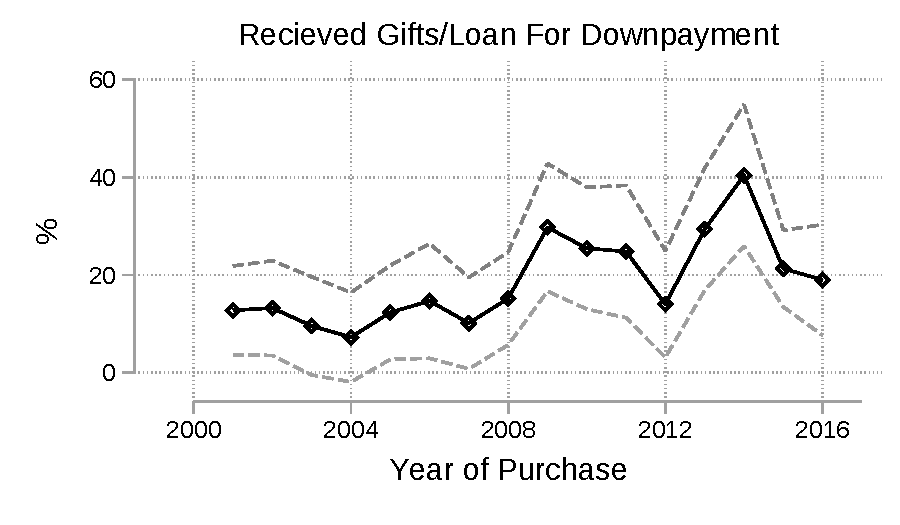
\includegraphics[width=0.5\textwidth]{../tabfig/descr/SHED_gift_scatter_SE_paper}%
	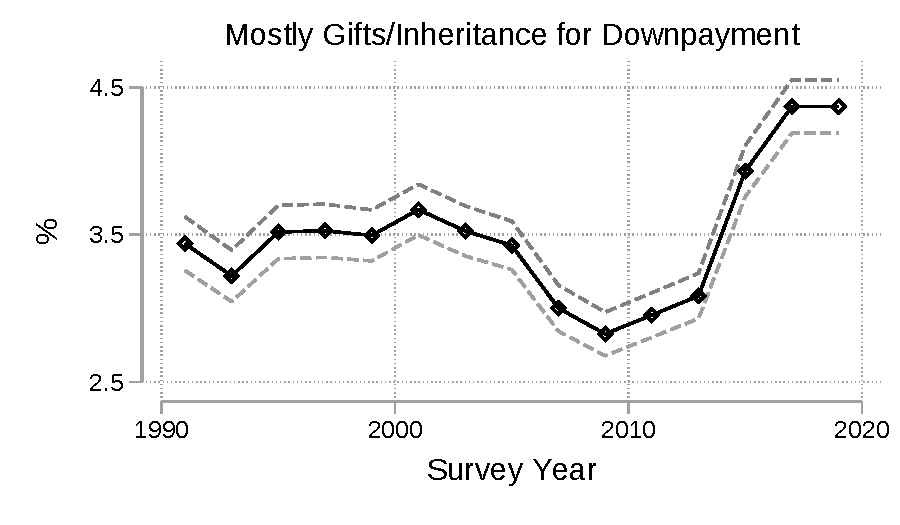
\includegraphics[width=0.5\textwidth]{../tabfig/descr/AHS_majorsourcedown_surveyyear_paper}%
	
	 {\begin{footnotesize} \textit{Notes:} The left panel uses data from the SHED with the sample restricted to current owners who report this being their first home. The right panel uses data from the AHS with the sample restricted to all owner-occupied units that did not indicate the sale of a previous home as the main source of funding.  Note that the left figure has year of purchase on the horizontal axis while the right figure has survey year. Dashed lines denote 95\% confidence intervals.\end{footnotesize}}
\end{figure}

\textit{SHED:} I use the 2015 and 2016 SHED, an annual cross-sectional survey conducted by the Federal Reserve, to observe the share of first-time owners who funded the down payment with a loan or gift from family or friends, by year of purchase. The sample includes 772 households with non-missing down payment and first-time ownership information. The results are plotted in the left panel of Figure \ref{fig:motivation}. The main observation is the large increase in the role of inter-vivos transfers for homeowners since 2001. From 2001 to 2007, only 10\% to 18\% of first-time buyers received transfers, while 20\% to 40\% received transfers after 2009.

\textit{AHS:} I use the 1991-2019 AHS, which surveys occupants of housing units, to construct a time series of whether homeowners primarily funded their down payment with gifts or inheritances (right panel). After excluding households who report sale of previous homes as a funding source, the sample includes about 50,000 observations each year. The series is relatively flat through the 1990s, followed by a sharp decline from 2005 to 2009---coinciding with the rise of low–down-payment mortgages---and a marked increase from 2013 onward. Because the horizontal axis reflects survey year rather than purchase year, minor fluctuations largely reflect variation among recent buyers, who make up a small share of all homeowners.

\subsection{Panel Study of Income Dynamics}\label{sec:PSID}
My main data source is the PSID, which follows a nationally representative sample of U.S. households and their descendants over time since 1968. The PSID is the only publicly available U.S. dataset that satisfies this paper's three requirements. First, it has detailed wealth, income, and housing data for both parents and adult children. Second, it has information about inter-vivos transfers from parents to children, unlike most register data. Third, it follows households over time, so we can observe the transitions from renting to owning and how these transitions relate to parental wealth.

I use data from 1999 to 2021. In 1999, the PSID started to collect detailed wealth data every other year. In most waves of the PSID, there is limited transfer data, and the main question is whether households received gifts or bequests over \$5,000 in the last two years. In 2013, the PSID collected more detailed transfer data in the Family Roster and Transfer Module. They asked parents how much they gave their children in the last calendar year and how much they had given over their lifetime for school, house purchases, or other purposes. Household characteristics such as age, gender, and education refer to the household head. I classify top-coded values as missing observations. All monetary variables are expressed in thousands of 2016 U.S. dollars.

\textit{Sample Selection:} Throughout this paper, the sample includes all households aged 25 to 84 in the PSID. All summary statistics are calculated using the provided family weights. I drop 1851 observations with missing housing values (which is set to zero for renters). The final sample has 18,075 households and 100,326 observations.

\textit{Matching Parents with Children:} I use the Parent/Child file from the PSID's 2013 transfer supplement. I can observe each household's reported transfers to and from parents and children. This leads to discrepancies, where the child and parent do not agree on the amount given from the parent to the child. For each child, I use the parent's reported transfer to that child. First, there may be some stigma about receiving transfers, which may induce receiving children to underreport. Second, in the model, parents determine the size of the transfer they give to their child. 

\textit{Definition of Transfers:} To measure the transfer receipt rate, I rely on the transfer supplement which asked all parent households whether they gave money, gifts, or loans of \$100 or more to each child in 2012. I follow the literature \citep[e.g.,][]{mcgarry2016dynamic} and treat all transfers as gifts. Since this paper focuses on transfers that (a) relate to housing and (b) are quantitatively meaningful, I ignore transfers below \$500. About 25\% of transfers are below this threshold, and ignoring them increases the conditional mean transfer from \$2,921 to \$3,960 and reduces the transfer receipt rate from 45\% to 22\%.\footnote{These transfer rates are relatively high and exceed those reported by \citealt{feiveson2019lifecycle} using the Survey of Consumer Finances (SCF). The PSID transfer supplement likely captures a broader range of transfers than the SCF, which deliberately focuses on substantial transfers. In addition, the SCF asks about transfers further back in time, increasing the risk of recall error and underreporting.}

In all other waves, there is a general question of gifts and inhertitances from people outside the household. We do not know the source of these transfers (e.g., they could be from friends or grandparents) and hence these do not know the extent to which these captures parental assistance. Nevertheless, they still capture some of the impact of transfer receipt on household decisions. I therefore include these variables in some of the empirical results, following \citet{Lee2018}.

Finally, why focus on inter-vivos transfers when most intra-family wealth transfers occur through bequests \citep[see e.g.,][]{feiveson2019lifecycle}? First, parental bequests are typically received after age 45, too late to affect young adults' transition into homeownership. Second, some bequests are given early and recorded as inter-vivos transfers. Third, inter-vivos transfers are often targeted to children's immediate liquidity needs, such as financing a home purchase, whereas bequests are often passive outcomes of unspent wealth. Fourth, while bequests dominate in aggregate terms, they are highly concentrated among wealthy households, whereas inter-vivos transfers are the main form of transfer for most parents \citep{yang2023financial}. Thus, inter-vivos transfers are more relevant for understanding early-life economic outcomes. 


\subsubsection{Descriptive Statistics: Who Receives Transfers?}
I now discuss descriptive statistics from the 2013 PSID sample for households aged 25 to 44 with an observed parent household. Table \ref{tab:descrstats} contains the means of variables, by age, wealth, homeownership, and transfer receipt. Though limited to households with observed parents, the sample appears reasonably representative. Average income by age closely matches estimates from the SCF \cite[see e.g.,][]{kuhn20162013}, though average wealth is slightly lower.

There are several main takeaways from the subgroup analysis. In 2012, 21\% of young households received a transfer, and transfers averaged \$3,960. Receivers have significantly richer parents, have similar wealth and income as nonreceivers, and are less likely to own. Receivers are more likely to transition from renting to owning, especially in the age groups where households are most likely to buy. The key determinant of transfer receipt seems to be parental wealth.

The first two columns of the top panel compare households by transfers receipt. The mean transfer is relatively high at \$3,960, and 21\% of households received transfers in the last year. The largest difference is parental wealth: transferring parents are 2.5 times as wealthy as nontransferring parents. Perhaps surprisingly, receivers are slightly richer than nonreceivers (\$108,000 vs. \$78,500), are more likely to be college-educated and white, and are one year younger. Receivers are slightly less likely to be homeowners (39\% vs. 43\%), reflecting the age difference and the tendency for college attendance to delay homeownership.

\begin{table}[tbp]
	\begin{adjustbox}{center}
		\small
		\def\sym#1{\ifmmode^{#1}\else\(^{#1}\)\fi}
		\begin{threeparttable}
			\singlespacing
			\caption{Descriptive Statistics (Means), Households Aged 25-44}\label{tab:descrstats}
			\begin{tabular}{l  r@{\hspace{1.\tabcolsep}}r r@{\hspace{1.\tabcolsep}}r r@{\hspace{1.\tabcolsep}}r r@{\hspace{1.\tabcolsep}}r}
				\toprule
				& \multicolumn{2}{c}{All}  &  \multicolumn{2}{c}{Renter}   & \multicolumn{2}{c}{Owner}    \\ \cmidrule(lr){2-3} \cmidrule(lr){4-5} \cmidrule(lr){6-7}
				Receiver 		& \multicolumn{1}{c}{No} & \multicolumn{1}{c}{Yes} & \multicolumn{1}{c}{No} & \multicolumn{1}{c}{Yes} & \multicolumn{1}{c}{No} & \multicolumn{1}{c}{Yes}    \\  \midrule
				\input ../tabfig/descr/descr_trsnf_disc_mean.tex
				\midrule
				Age                    & \multicolumn{2}{c}{25-31} & \multicolumn{2}{c}{32-38}  & \multicolumn{2}{c}{39-44}   \\ \cmidrule(lr){2-3} \cmidrule(lr){4-5} \cmidrule(lr){6-7}
				Receiver       & \multicolumn{1}{c}{No} & \multicolumn{1}{c}{Yes} & \multicolumn{1}{c}{No} & \multicolumn{1}{c}{Yes} & \multicolumn{1}{c}{No} & \multicolumn{1}{c}{Yes}    \\ 
				 \midrule
				\input ../tabfig/descr/descr_trsnf_age_mean.tex
				\midrule
				Wealth Tertile                    & \multicolumn{2}{c}{Tertile 1}  & \multicolumn{2}{c}{Tertile 2}  & \multicolumn{2}{c}{Tertile 3}    \\ \cmidrule(lr){2-3} \cmidrule(lr){4-5} \cmidrule(lr){6-7}
				Receiver       & \multicolumn{1}{c}{No} & \multicolumn{1}{c}{Yes} & \multicolumn{1}{c}{No} & \multicolumn{1}{c}{Yes} & \multicolumn{1}{c}{No} & \multicolumn{1}{c}{Yes}    \\ 
				\midrule
				\input ../tabfig/descr/descr_trsnf_wlt_mean.tex
		\bottomrule
			\end{tabular}
		\end{threeparttable}
	\end{adjustbox}
	{\begin{footnotesize}\begin{flushleft}\vspace{-0.1in}%
		\textit{Notes:} Data from the PSID Transfer, Individual, and Family modules. Weighted using family weights. Transfer, wealth, and income measured in 1000s of 2016 USD. Table \ref{tab:vardef} in the Appendix provides variable codes of the main variables.
	\end{flushleft}\end{footnotesize}}		
	\end{table}
	
Next, I break the sample down by ownership. Homeowners are both wealthier and have wealthier parents than renters. Renters and owners receive transfers at about the same rate and size. Receivers are more likely to switch from renting to owning: 21\% of receiving owners rented two years ago, compared to 14\% of nonreceiving owners.

Next, I break the sample into three age groups from 25 to 44. We see that households' wealth, income, and homeownership rates increase with age. Notably, among 29-to-32-year-olds, homeownership is more common among transfer recipients (40\%) than nontransfer recipients (32\%). Furthermore, receivers are not only more likely to own, but also to be recent homeowners: 21\% of receiving owners are new homeowners versus 13\% of nonreceiving owners. 

\subsubsection{Transfer Sizes}
For additional detail on the transfer variables, I plot kernel density estimates in Figure \ref{fig:PSID_transfer_to_renters}, for renters in $t$, separated by whether they own or rent in $t+2$, for the two transfer definitions. There are two takeaways. First, households who transition to ownership receive larger transfers on average, under both transfer measures. Second, the transfers in the transfer supplement are much smaller than than those in the gift/inheritance question. Indeed, the median parental transfer is about \$1k, the mean about \$3k, and the 95th percentile is at \$10k, compared to the median gift/inheritance of \$25k, mean of \$60k, and a 95th percentile of about \$130k.

\begin{figure}[tb]
	\caption{Transfer Sizes to Renters by Transition to Ownership}\label{fig:PSID_transfer_to_renters}
	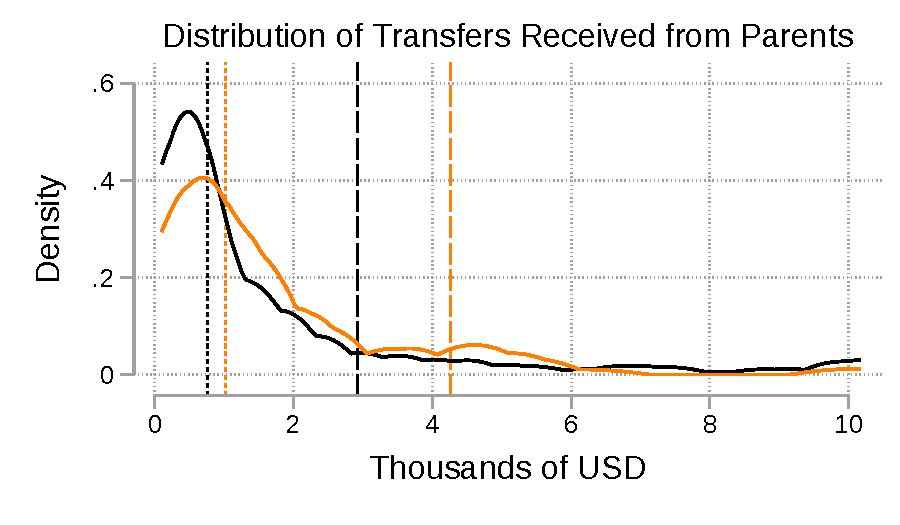
\includegraphics[width=0.5\textwidth]{../tabfig/descr/PSID_transfers_renters_transfers.pdf}% 
	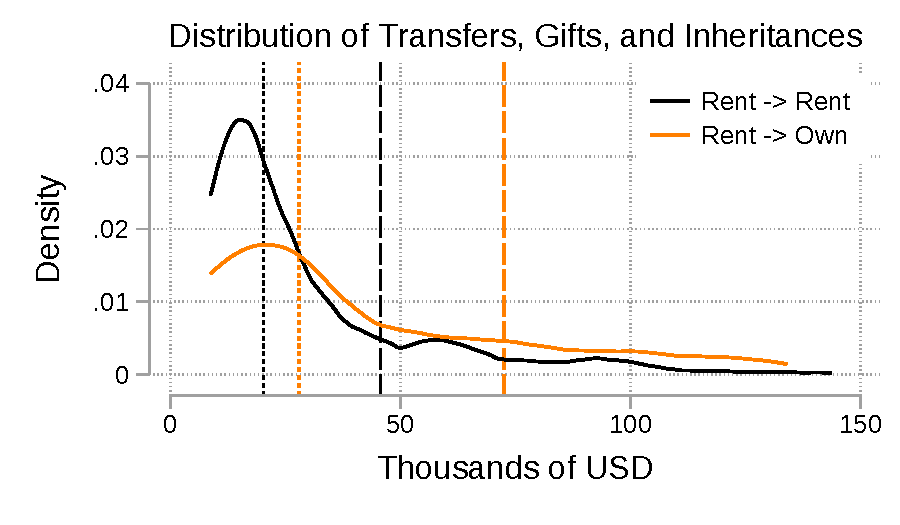
\includegraphics[width=0.5\textwidth]{../tabfig/descr/PSID_transfers_renters_inheritance.pdf}%
	
	 {\begin{footnotesize} \textit{Notes:} The left panel uses the transfers, gifts, and inheritance variable which is available in all waves of the PSID while the right panel uses the parental transfer data only available in the 2013 transfer supplement. See main text for a discussion. Vertical dotted and dashed lines denote the median and means, respectively. All estimates are weighted and omit the top 5\% of transfer sizes. \end{footnotesize}}
\end{figure}

While the PSID allows us to observe transfers and changes in housing tenure over time, it has several limitations. First, the transfer supplement captures transfers only in 2012, while the PSID is collected biennially, leading to undercounts of both transfer rates and amounts. Second, in the gift/inheritance question, the source of the transfer is unknown. Third, it is unclear whether intra-family loans are consistently reported or repaid.

\subsection{Parental Resources and Housing Outcomes in the Data}\label{sec:dataregr}

I now utilize microdata from the PSID to examine the empirical association between parental financial resources on housing outcomes. The sample is limited to households aged 25 to 44 to focus on the housing choices of young adults. I use the sum of parental net worth and income (denoted as wealth) to measure parents' financial resources in all specifications for two reasons. First, this is consistent with models of altruism, as the one used later in the paper. Second, since parents' wealth and income are highly correlated and I have few observations---fewer than 1,000 for many specifications---the standard errors are large when both are included.

\subsubsection{Transfers and the Transition into Homeownership}
Since many papers have already estimated the relationship between parental transfers and transitions into homeownership (e.g.\ \citealp{wold2024housing}; \citealp{Blickle2019}; \citealp{benetton2022dynastic}; \citealp{Lee2018}), I replicate these regressions to highlight the association between transfer receipt and rent-to-own transitions, but relegate the full results to Appendix~\ref{app:rent_to_own}. Receiving a parental transfer above \$500 is associated with a 1.2 percentage point increase in the probability of becoming a homeowner (not statistically significant), after controlling for household characteristics. Receiving large transfers above \$10,000 is associated with a 7.9 percentage point increase in the probability of becoming a homeowner ($p<0.1$), even after including household fixed effects. These are sizable effects relative to the baseline rent-to-own transition probability of about 18\% during the sample period.


\subsubsection{Households with Wealthier Parents Retain Ownership}
While most research focuses on the transition into ownership, I now focus on the challenge of retaining it.

\begin{figure}[tb]
	\captionsetup[subfigure]{aboveskip=-1pt}
	\caption{Retaining Homeownership}\label{fig:homeowner_exit}
	\begin{subfigure}{0.33\textwidth}%
		\caption{Retaining Ownership}\label{fig:owner_hazard}%
		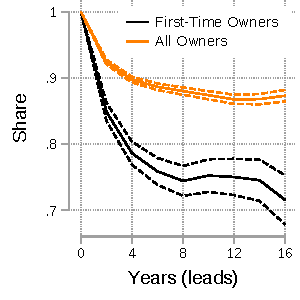
\includegraphics[width=\textwidth]{../tabfig/descr/PSID_ownerexit.pdf}% 
	\end{subfigure}%
	\hfill
	\begin{subfigure}{0.33\textwidth}%
		\caption{All Owners}\label{fig:coef_allowner}%
		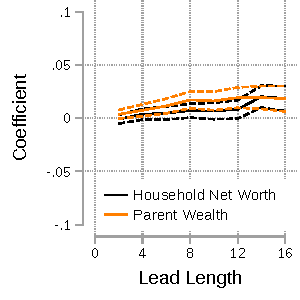
\includegraphics[width=\textwidth]{../tabfig/descr/PSID_coefowner.pdf}% 
	\end{subfigure}%
	\hfill
	\begin{subfigure}{0.33\textwidth}%
		\caption{First-Time Owners}\label{fig:coef_ftowner}%
		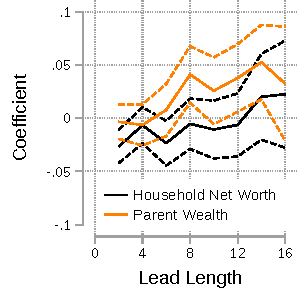
\includegraphics[width=\textwidth]{../tabfig/descr/PSID_coefftowner.pdf}% 
	\end{subfigure}%
	
	\caption*{\footnotesize \textit{Notes:} The left panel shows the share of current owners who remain owners in future years. The center and right panels show the estimated coefficients from Eq.~\ref{eq:regmaintain}, with dashed lines indicating 90\% confidence intervals. See main text for details.}
\end{figure}

First, the left panel of Figure \ref{fig:owner_hazard} plots the share of owners aged 25 to 44 in year $t$ who remain owners in period $t+\Delta$. Among first-time owners, only 80\% have retained ownership four years later. For non-first-time owners, there is still a marked decrease though it is more muted, after four years about 10\% of all owners will be renting. 

To understand which variables predicts retainment of ownership, I estimate
\begin{equation}	\label{eq:regmaintain}
	\Pr\left(Own_{i,t+\Delta}=1|Own_{i,t}=1\right)
	= \beta\ln(NetWorth_{i,t}) + \zeta\ln(ParWealth_{i,t})
	  + \gamma' X_{i,t} + \varepsilon_{i,t},
\end{equation}
where $Own_{i,t+\Delta}=1$ denote ownership at time $t+\Delta$, $\beta$ and $\zeta$ measure the effects of log household net worth and parental wealth, respectively. The vector of control variables  $X_{i,t}$ consists of log household income, log household size, age, parental age, and dummies for  education, marital status, race, household composition changes, and state and year fixed effects.  The sample is limited to households aged 25 to 44. These regressions are motivated by \cite{bond2021role}, who estimate similar equations in the PSID and the Health and Retirement Study. Figures \ref{fig:coef_allowner} and \ref{fig:coef_ftowner} plot the two coefficients of interest over different time horizons.

Two results stand out. First, parental wealth is at least as predictive as household net worth at all horizons, although the difference is never statistically significant. Second, the effect of current parental wealth grows with the time horizon. For instance, a 10\% increase in parental wealth raises the probability of retaining ownership after eight years by 0.45 percentage points among first-time owners. I return to these results later as part of the model validation.


\subsubsection{Households with Wealthier Parents Are Less Delinquent} 
One potential roadblock to maintaining ownership is mortgage delinquency, as missed payments can lead to distressed or forced sales. I show that households with wealthier parents are less likely to fall behind on their mortgages, despite purchasing more expensive homes. The PSID has collected mortgage delinquency data since 2009; about 2\% of owners aged 25 to 44 report being behind.

To examine what predicts mortgage delinquency, I estimate: 
\begin{equation}\label{eq:regbehind}
\Pr(Behind_{i,t+2}) = \beta\ln(NetWorth_{i,t}) + \zeta\ln(ParWealth_{i,t}) + \gamma' X_{i,t} + \varepsilon_{i,t},
\end{equation}
using the same control variables as in the previous regression. Table~\ref{tab:hypo} reports the estimated coefficients on parental wealth ($\zeta$); full results appear in Appendix Table~\ref{tab:hypo_long}.  

I first limit the sample to first-time buyers to focus on distress among new owners. In a univariate regression, a 10\% increase in parental wealth is associated with a 0.07 percentage point decrease in the probability of being behind on mortgages two years later ($p<0.1$) With the full set of controls, the effect increases slightly, though it is no longer statistically significant. These magnitudes are economically meaningful since 1.6\% of first-time owners are behind on their mortgage.In Columns 3 to 5, I expand the analysis to include all owners who are currently not behind, increasing the sample sizes and allowing us to include household fixed effects. In these specifications, a 10\% increase in parental wealth is associated with a 0.09 percentage point decrease in delinquency risk in the univariate OLS regression ($p<0.001$), a 0.02 percentage point decrease in the multivariate OLS regression (not significant), and a 0.07 percentage point decrease in the fixed effects regression ($p<0.1$).

\begin{table}
	\centering
	\begin{threeparttable}
		\caption{Parental Wealth and Future Mortgage Delinquencies}
		\label{tab:hypo}
		\small 
				{
\def\sym#1{\ifmmode^{#1}\else\(^{#1}\)\fi}
\begin{tabular}{l*{5}{c}}
\toprule
                &\multicolumn{1}{c}{(1)}&\multicolumn{1}{c}{(2)}&\multicolumn{1}{c}{(3)}&\multicolumn{1}{c}{(4)}&\multicolumn{1}{c}{(5)}\\
                &\multicolumn{1}{c}{OLS}&\multicolumn{1}{c}{OLS}&\multicolumn{1}{c}{OLS}&\multicolumn{1}{c}{OLS}&\multicolumn{1}{c}{FE}\\
\midrule
\;Parental Wealth&   -0.007\sym{+}  &   -0.010         &   -0.009\sym{***}&   -0.002         &   -0.007\sym{+}  \\
                &  (0.004)         &  (0.008)         &  (0.002)         &  (0.002)         &  (0.004)         \\
\midrule
N               &      957         &      623         &    5,369         &    4,669         &    4,669         \\
Outcome (mean)  &    0.016         &    0.016         &    0.024         &    0.020         &    0.020         \\
First-Time Buyers Only&        Y         &        Y         &        N         &        N         &        N         \\
Other Controls  &        N         &        Y         &        N         &        Y         &        Y         \\
\bottomrule
\end{tabular}
}

	
	\end{threeparttable}
	{\begin{footnotesize}\begin{flushleft}
		\textit{Notes:} The estimated association between parental wealth and the probability of behind on mortgage payments in the next period from regressions using specification \ref{eq:regbehind}. See Appendix Table~\ref{tab:hypo_long} for all results. Standard errors in parentheses, clustered at the household level. \textsuperscript{+}$p<0.10$, \textsuperscript{*}$p<0.05$, \textsuperscript{**}$p<0.01$, \textsuperscript{***}$p<0.001$.
		\end{flushleft}\end{footnotesize}}	
\end{table}

Overall, the probability of falling behind on mortgage payments declines with parental wealth, even after controlling for a wide range of household characteristics. This highlights a novel channel through which parental resources help new homeowners retain ownership after purchase.


\subsubsection{Owners with Wealthy Parents Don't Downsize in Unemployment}\label{sec:eventstudy}
Distressed and forced home sales are costly and often triggered by unemployment \citep{kermani2021racial,hsu2018unemployment}. To test whether parental wealth mitigates this risk, I perform a simple event study of how unemployment affects the likelihood of downsizing.

The exercise follows \cite{Chetty2007} closely. The outcome of interest is the change in log housing consumption, which is set to zero for households who do not move. For movers, housing consumption is defined as yearly rent while renting and as imputed rent for owners, set to 5\% of the market value \citep{Davis2008}. The sample is limited to household heads who experience only one unemployement spell between ages 25 and 44. I divide the sample by whether a household's parents were in the top parental wealth quartile at the time of unemployment and compare the two groups' housing consumption growth at unemployment. The results are displayed in Figure \ref{fig:housinggrowthrates}. Among households with non-wealthy parents, housing consumption falls by about 5\% during unemployment ($p<0.05$). In contrast, households with wealthy parents see a slight increase (not significant)in housing consumption during unemployment.\footnote{In Appendix \ref{app:eventstudy_details}, I also report the results of a formal event study using the same set of controls as in the previous regressions.}  I return to these results later as part of the model validation.

\begin{figure}
	\caption{Event Study: Housing Consumption at Unemployment by Parental Wealth}\label{fig:housinggrowthrates}
	\noindent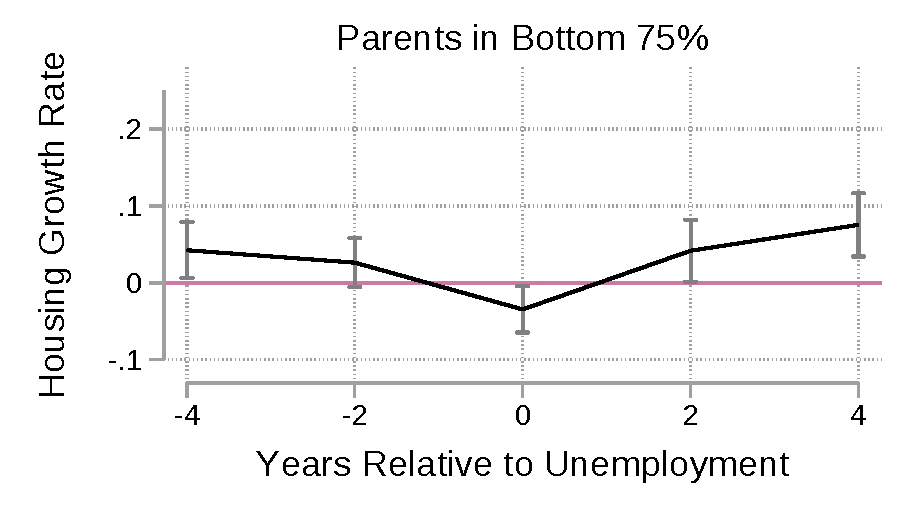
\includegraphics[width=0.5\textwidth]{../tabfig/descr/PSID_housinggrowthpoor_both}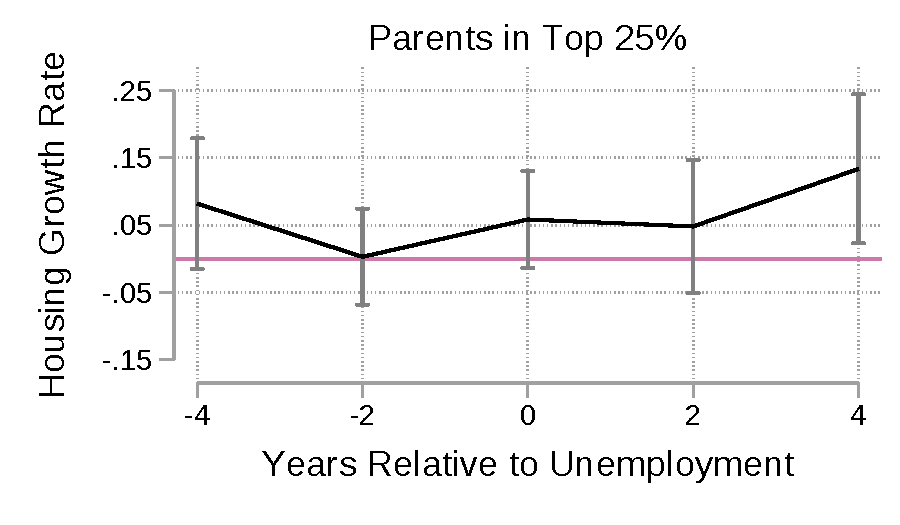
\includegraphics[width=0.5\textwidth]{../tabfig/descr/PSID_housinggrowthrich_both}

	{\begin{footnotesize} \textit{Notes:} Solid lines denote means, and bars denote the 95\% confidence interval. The sample consists of households aged 25-45 with exactly one unemployment spell and without changes in head and/or spouse in the four years before and after unemployment. \end{footnotesize}}
\end{figure}

\subsection{Taking Stock of the Data}
Taking stock, we have seen that parental transfers have become more important for young homeowners over the past two decades. About 20\% of young households receive transfers from their parents in a given year, and recipients have wealthier parents. Recipients are more likely to transition from renting to owning, even after conditioning on a rich set of covariates. Parental wealth is also positively associated with maintaining homeownership. Households with richer parents are less likely to fall behind on mortgages and less likely to downsize during unemployment spells. These results suggest that homeowners with wealthy parents find illiquidity of homeownership less problematic.

\subsection{Transfers and Taxes}
In the United States, transfers and bequests are subject to taxation due to the estate tax. Taxes are paid by the giver, not the recipient. In 2024, an individual can give \$13.61 million before they start owing gift taxes. However, individuals have to file if they give transfers above \$18,000 (in 2024) to any one individual within a calendar year. Thus, the gift tax is irrelevant for the vast majority of households, as it applies only once lifetime transfers---including bequests---exceed \$13.61 million.


\section{A Quantitative Model of Parental Transfers and Homeownership}\label{sec:model}
This section describes my life-cycle model of housing choices with overlapping generations, idiosyncratic earnings risk, and altruistic inter-vivos transfers from parents to their offspring (``children''). To answer how important parental transfers are for housing outcomes, I combine two models: altruism without commitment and illiquid housing. 

Altruism without commitment is a standard model of intergenerational family interactions (e.g., \cite{Altonji1997a,Barczyk2018}). Altruistic parents, deriving utility from their child's utility, influence their child's consumption and housing choices through nonnegative transfers. The lack of commitment aligns with empirical transfer patterns and generates strategic behavior, as both children and parents internalize the effect of their choices on each other's future choices. The central theoretical prediction is that wealthy parents transfer to children with high marginal utility of wealth, typically poor or borrowing-constrained households \citep{Chu2020,Barczyk2020}.

The second model component is illiquid homeownership. Without illiquidity, transfers mainly relax mortgage constraints, as has been the focus in empirical literature (e.g., \cite{Blickle2019,Engelhardt1998,Guiso2002,Lee2018}). With illiquidity, we get a two-asset model where portfolio composition matters for transfers. Specifically, homeowning children with low liquid wealth (``house rich but cash poor'') have high marginal utility of wealth, strengthening parental transfer motives and, thus, the child's homeownership motive. Finally, while illiquid housing makes selling costly, wealthy parents can offer partial insurance, thus reducing the risk of costly liquidation or downsizing.

These two housing frictions---borrowing constraints and illiquidity---are not only theoretically important, but also empirically relevant. In the SHED, 57\% of renters could not afford a down payment or did not qualify for a mortgage, while 26\% said that renting was more convenient and 23\% cited planning to move as reasons for renting. 

\subsection{Demographics, Preferences, and Technologies}
Time is discrete and finite. Each period consists of two years. At the beginning of each period, a constant mass of new households enters and exits the economy. The only economic agents in the model are households.

\textit{Demographics:} Households enter the economy at age $a=25$ and die at age 83. The life cycle is illustrated in \ref{fig:overview}. A family consists of one adult child $c$ household (age 25 to 53) and a parent $p$ household (age 55 to 83) with an age gap of 30. Thus, children have new children at age 30, but new children are economically inactive until age 25. Each parent-child pair overlaps for 15 periods (30 years), and only two households are economically active in any dynasty at a time. Three events happen simultaneously when a child household becomes 55. First, the household's parent dies (at age 85). Second, the child transitions to become a parent household. Third, the child of the child becomes economically active as a child household.

\begin{figure}\begin{center}
	\caption{Life Cycle of Three Generations in a Dynasty }\label{fig:overview}
	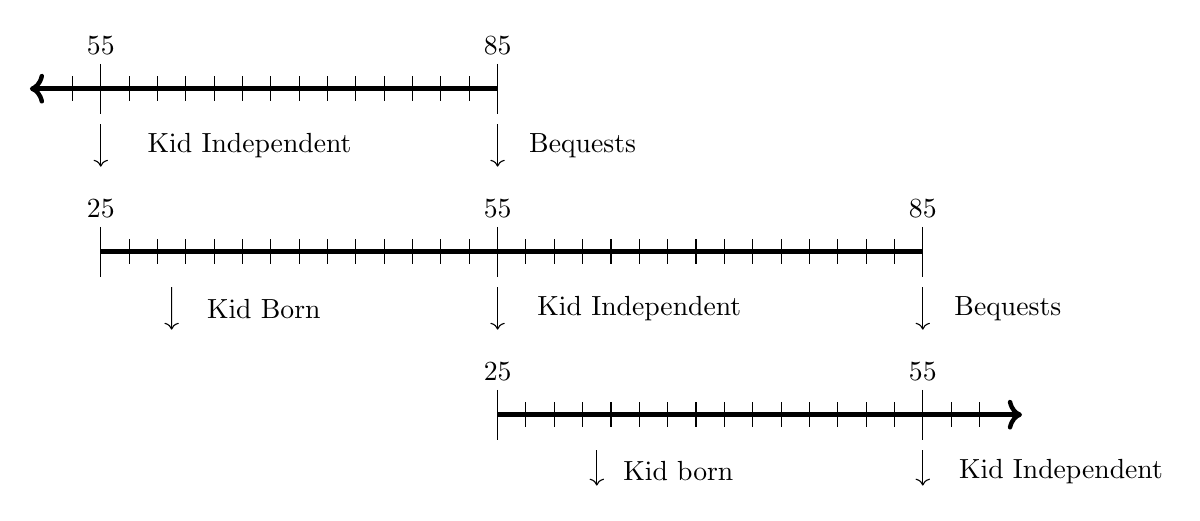
\begin{tikzpicture}[scale=0.9]
	% Iniold
	\foreach \x in {0,1,2,3,...,30}
	{
		\coordinate (C\x) at ($(0,0cm)+(\x*0.4cm,-0cm)$) {};
	}
	\foreach \x in {0,1,2,3,...,15}
	{
		\draw ($(C\x)+(0,5pt)$) -- ($(C\x)-(0,5pt)$);
	}
	\draw[ultra thick,arrows=<-] ($(C1)-(1,0)$) -- (C1) -- (C15);
	\draw ($(C1) + (0,10pt)$) -- ($(C1) - (0,10pt)$);
	\draw ($(C15) + (0,10pt)$) -- ($(C15) - (0,10pt)$);
	\node at ($(C1)+(0,4ex)$) {55};
	\node at ($(C15)+(0,4ex)$) {85};
	
	% Middle
	\foreach \x in {1,2,...,33}
	{
		\coordinate (A\x) at ($(0,-2.3)+(\x*0.4cm,0)$) {};
	}
		\foreach \x in {1,2,...,30}
	{
		\draw ($(A\x)+(0,5pt)$) -- ($(A\x)-(0,5pt)$);
	}
	\draw[ultra thick] (A1) -- (A30);
	\draw ($(A1) + (0,10pt)$) -- ($(A1) - (0,10pt)$);
	\draw ($(A15) + (0,10pt)$) -- ($(A15) - (0,10pt)$);
	\draw ($(A30) + (0,10pt)$) -- ($(A30) - (0,10pt)$);
	
	\node at ($(A1)+(0,4ex)$) {25};
	\node at ($(A15)+(0,4ex)$) {55};
	\node at ($(A30)+(0,4ex)$) {85};
	
	%Young
	\foreach \x in {1,2,3,...,33}
	{
		\coordinate (B\x) at ($(0,-4.6cm)+(\x*0.4cm,0cm)$) {};
	}
	\foreach \x in {15,16,17,...,32}
	{
		\draw ($(B\x)+(0,5pt)$) -- ($(B\x)-(0,5pt)$);
	}
	\draw[ultra thick,arrows=->] (B15) -- (B32) -- ($(B31)+(1,0)$);
	\draw ($(B15) + (0,10pt)$) -- ($(B15) - (0,10pt)$);
	\draw ($(B30) + (0,10pt)$) -- ($(B30) - (0,10pt)$);
	
	\node at ($(B15)+(0,4ex)$) {25};
	\node at ($(B30)+(0,4ex)$) {55};

	%% Labels
	
	\draw[arrows=->] ($(C1) - (0,0.5)$) -- ($(A1) + (0,1.2)$);
	\draw[arrows=->] ($(C15) - (0,0.5)$) -- ($(A15) + (0,1.2)$);
	\node[align=left]  (kid) at ($(C6)!0.35!(A6)+ (0.1,0)$ ) {Kid Independent};
	\node[align=left]  (beq) at ($(C18)!0.35!(A18)$) {Bequests};
	
	\draw[arrows=->] ($(A3) - (-0.2,0.5)$) -- ($(B18) + (-5.8,1.2cm)$) ;
	\node[align=left] (newkid) at ($(A6)!0.35!(B6) + (0.3,0)$)  {Kid Born};
	\draw[arrows=->] ($(A15) - (0,0.5)$) -- ($(B15) + (0,1.2)$);
	\node[align=left]  (kid) at ($(A20)!0.35!(B20)$) {Kid Independent};
	\draw[arrows=->] ($(A30) - (0,0.5)$) -- ($(B30) + (0,1.2)$);
	\node[align=right]  (beq) at ($(A33)!0.35!(B33)$) {Bequests};
	
	\draw[arrows=->] ($(B18) - (-0.2,0.5)$) -- ($(B18) + (0.2,-1.cm)$) ;
	\node[align=left] (newkid) at ($(B18) + (1.35,-0.8)$)  {Kid born};
	\draw[arrows=->] ($(B30) - (0,0.5)$) -- ($(B30) - (0,1)$);
	\node[align=right]  (beq2) at ($(B33) + (0.75,-0.8)$) {Kid Independent};		
	\end{tikzpicture}
\end{center}
\end{figure} 

\textit{Preferences and Altruism:} Parents and children have time-separable expected utility with a discount factor of $\beta$. Households maximize expected utility, and the per-period utility function for children is
\begin{equation}
U_c(c_c,h_c) = u(c_c,h_c) = \frac{\left(c_c^\xi s(h_c)^{1-\xi}\right)^{1-\gamma}-1}{1-\gamma},
\end{equation}
where $c$ is consumption, $h$ is housing, $\gamma$ is the coefficient of relative risk aversion, and $\xi$ measures the relative importance of consumption to housing services. The within-period Cobb-Douglas aggregator imposes a constant desired expenditure share on housing services, roughly consistent with empirical evidence (e.g., \cite{davis2011household}). The function $s(h)$ allows utility to depend on ownership:
\begin{equation}
s(h) = \begin{cases}
h & \text{ if renting}, \\
\chi h & \text{ if owning}.
\end{cases}
\end{equation}
The parameter $\chi$ measures the owner-occupied utility premium, reflecting any additional benefits derived from owner-occupation, such as stability or ownership rights.

The parent's utility also depends on the altruistic utility derived from the child:
\begin{equation}
U_p(c_p,h_p,c_c,h_c) = u(c_p,h_p) + \eta u(c_c,h_c),
\end{equation}
where $\eta$ measures the intensity of the parent's altruism towards the child. As usual with altruism, the parent also derives altruistic utility after death.

\textit{Intergenerational Transfers:} In the last period before death, the parent can leave a bequest, which the child receives in the next period. In all other periods, the parent can give inter-vivos transfers of a nonnegative amount, $t_p$, that the child receives immediately.

\textit{Housing:} Households can obtain housing services by renting or owning. They can rent housing of size $h_r$ or own houses of size $h_o$, with one size available for each tenure choice for tractability. The unit price of housing is $p$, and $q$ denotes the rent-to-price ratio. I assume that prices are constant for tractability, but I model aggregate house price risk as in \cite{Corbae2015} in Appendix \ref{sec:robust_pricerisk} and find that the quantitative results are almost unchanged. Homeowners incur proportional maintenance and depreciation costs $\delta$. Illiquidity is captured by proportional adjustment and moving costs on owner-occupied housing, as in \cite{Yang2009}:
\begin{equation}\label{eq:transcost}
adj(h_{a+1},h_a) = \begin{cases}
m_b p h_{a+1} & \text{if } h_{a}=h_r\mathbin{\&} h_{a+1}= h_o, \\
m_s p h_a 	& \text{if } h_a = h_o\mathbin{\&}h_{a+1}=h_r, \\
0 & \text{if } h_{a+1} = h_a,
\end{cases}
\end{equation} where $m_s$ and $m_b$ denote selling and buying costs, respectively. A household enters the period house $h_a$, while $h_{a+1}$ is the house chosen in this period. 

\textit{Financial Market:} Households can save in one-period bonds that pay the risk-free rate $r$. Households can also borrow in one-period risk-free bonds (``mortgage'') at an interest rate $r + r^m$, where $r^m$ is the mortgage premium. However, only owners may borrow, subject to a loan-to-value (LTV) constraint:
\begin{align*}
\begin{cases}
b\ge - LTV \times p h_{a+1} & \text{if } h_{a+1} = h_o, \\ 
b\ge 0 & \text{if } h_{a+1} = h_r.
\end{cases}
\end{align*}

In the U.S., borrowers making low down payments typically pay for private mortgage insurance (PMI) until their home equity surpasses a threshold \citep{goodman2017sixty}. I model this as an extra fee $r^{pmi}$ that households must pay until they reach the $\overline{PMI}$ threshold. Since the mortgage premium is positive, households never hold both a mortgage and savings in the bond, and the interest rate on the net bond $b$ is given by
\begin{equation}\label{eq:rb}
r(b) = \begin{cases}
r & \text{ if } b \ge 0, \\
r +r^m & \text{ if } -\overline{PMI}\times p\times h_o < b \le 0, \\
r +r^m +r^{pmi}& \text{ if } b \le -\overline{PMI}\times p\times h_o.
\end{cases}
\end{equation}

\textit{Net Worth:} Let $x$ denote net worth, defined as the sum of the bond position and the value of owner-occupied housing.

\textit{Income Endowment:} Households are endowed with an income process with a deterministic life-cycle profile $l_a$. Children face persistent idiosyncratic age-dependent productivity shocks $y_{i,a}\in\mathcal{Y}_a=\{y_1,\dots,y_{N_y}\}$, which follow a Markov chain, where $\pi_a(y'|y)$ is the probability of switching from state $y$ to $y'$ at age $a$. Parents face no income uncertainty. Consequently, income of household $i$ at age $a$ is given by
\begin{align}
w_{i,a} &= l_ay_{i,a} \; \forall a\in\{25,27,\dots,53\}, \label{eq:wk} \\
w_{i,a} &= l_a \; \forall a\in\{55,57,\dots,83\}. \label{eq:wp}
\end{align}
I assume that parents face no income risk for simplicity, consistent with the decrease in income risk with age \citep{Sanchez2020} and the fact that much of retirement income---such as Social Security and defined benefit pensions---is relatively certain. Furthermore, this paper focuses on the role of parental transfers for children' housing choices, where parental income risk is not a first-order concern. However, in Appendix \ref{sec:robust_incomerisk}, I show that parental income and health expenditure risks do not meaningfully change my results.

\textit{Initial Conditions of the New Child:} When children enter the economy at age $a_c=25$, their initial net worth $x_{25}$ and productivity $y_{25}$ are stochastic but correlated with the parent's wealth $x_{53}$ and productivity $y_{53}$ according to $x_{25}, y_{25} \sim F(x_{53}, y_{53})$. The initial net worth is not funded by parental transfers, though children can receive transfers in the first period. While I abstract from parental investment in human capital—an important driver of intergenerational persistence \citep[see e.g.,][]{Daruich2018,Lee2019}—the function $F$ matches observed correlations in wealth and income, ensuring realistic transfer motives. All households begin as renters.

\textit{Timing:} The child's productivity is realized first. If the dynasty has a newly economically active child, they also realize their initial wealth and productivity. The decision problem then proceeds in two stages. First, the parent chooses consumption $c_p$, housing $h_p$, savings position $b_p$, and nonnegative inter-vivos transfers $t_p$. After observing the parent's choices, the child in the second stage chooses consumption $c_c$, housing $h_c$, and savings $b_c$. The parent acts first, so that transfers can alleviate LTV constraints and to comply with U.S. mortgage regulations, which require gifts to be deposited before loan approval.

\subsection{Household Decision Problems}
I now present the recursive formulation and the decision problems. For clarity, I omit individual subscripts and apply a prime superscript to all $a+1$ variables.

\textit{State Variables and Setup:} Let $\mathbf{g}_p$ and $\mathbf{g}_c$ denote the vectors of the parent's and child's policy functions, respectively.

A parent $p$'s state variables are child's wealth $x_c\in X=[0,\infty)$, parent's wealth $x_p\in X$, child's housing $h_c\in H = \{h_r,h_o\}$, parent's housing $h_p\in H$, child's productivity $y_c\in Y_a=\{y_1,\dots,y_{N_y}\}$, and age $a_c\in A_c\in\{25,27,\dots,53\}$. The parent's state variable vector is $\mathbf{s}_p\equiv\left(x_c,x_p,y_c,h_c,h_p,a_c\right)$. 

The child's state space differs because the parent's choices influence the child's decisions. The child is indifferent to receiving an additional unit of wealth or transfers, focusing only on total wealth (including transfers), $\tilde x_c\equiv x_c+t_p$. Furthermore, the parent's current wealth and housing are redundant; the child cares only about the parent's bond and housing choices, since future transfers depend on the parent’s next-period resources.  The child's state variable vector is $\mathbf{s}_c=\left(b_p',h'_p,x_c+t_p,y_c,h_c,a_c\right)$. 




\textit{Decision Problems:} 
I now show the decision problems for a dynasty at age $a_c < 53$. For simplicity, I assume the child is a renter choosing to become an owner, while the parent remains a renter. 

\textit{Child - Second Stage:} The child, conditional on becoming a new owner ($h_c=h_r,h'_c=h_o$), chooses consumption and bonds to maximize expected utility:
\begin{equation}\label{eq:Vk}
\begin{split}
 V_c(\mathbf{s}_c;\mathbf{g}_p)^{own} = \max_{c_c,b'_c,h'_c=h_o} & u(c_c,h'_c) + \beta \E_{y_c}\left[V_{c}(\mathbf{s}_c';\mathbf{g}_p) \right] \\ 
 \text{s.t.}\quad & 	b'_c = \tilde x_c + w_c - c_c - p h'_c - m_b p h'_c \\
 & x_c' = b'_c(1+r(b'_c)) + p h'_c(1-\delta) \\
 & b_c' \ge - LTV p h'_c. 
\end{split}
\end{equation}
The first constraint is the budget constraint, which determines the net bond position as available resources (net worth, transfers, and income) minus expenditures (consumption, purchase price, and purchase cost). The second constraint is the law of motion for net worth, which is the sum of the bond position and housing wealth after maintenace costs. The third constraint is the LTV constraint. We see that a transfer $t_p$ can move the child away from the LTV constraint by increasing the bond position $b_c'$, holding consumption and housing fixed. The expectation is conditional on the child's current productivity. The child's value functions are conditional on the parent's policy functions because the child's choices depend on the parent's choices.

For the other three possible housing choices (remain renting, remain owning, and own to rent), the problem is similar, but with appropriate changes to the budget equation, law of motion, and borrowing constraint. Finally, the child must choose between the two housing options:
\begin{equation}
	V_c(\mathbf{s}_c) = \max_{h_c'} \left\{V_c(\mathbf{s}_c)^{rent},V_c(\mathbf{s}_c)^{own}\right\}.
\end{equation}

\textit{Parent - First Stage:} The parent, conditional on remaining a renter ($h_p=h'_p=h_r$), chooses consumption, transfers, and bonds to maximize expected utility:
\begin{equation}\label{eq:Vp}
\begin{split}
V_p(\mathbf{s}_p;\mathbf{g}_c)^{rent} = \max_{c_p,b_p',t_p} & u(c_p,h'_p) + {\eta} u\left (c_c^*({\mathbf{s}_c}),h_c'^*({\mathbf{s}_c})\right ) + \beta \E_{y_c} \left[V_{p}({\mathbf{s}_p';\mathbf{g}_c})\right] \\
\text{s.t.}\quad & b'_p = x_p + w_p - c_p - t_p - q p h_p'\\
& x_p' = b'_p(1+r(b'_p)) \\
& t_p\ge0, \\
& b_p'\ge 0. \\
\end{split}
\end{equation}
The first constraint is the budget constraint, which determines the net bond position as available resources (net worth and income) minus expenditures (consumption, transfers, and rent). For renters, next-period wealth is simply given by the bond position. The third and fourth constraints impose that transfers be nonnegative and that renters may not borrow, respectively. Finally, the parent chooses whether to rent or own.

\textit{Next-Period States:}
When making decisions, households consider how their choices will impact future states, as we can see from the next-period state vectors. For example, the parent internalizes that their next-period state includes the child's next-period wealth and housing, which are functions of the child's current choices, which in turn depend on the parent's current choices:
\begin{equation}
	\mathbf{s}_p' = \left(x_c'^{*}({\mathbf{s}_c}),x_p',y_c',h'^*_c({\mathbf{s}_c}),h'_p,a_c'\right).
\end{equation}
Similarly, the child knows that their next-period state includes the parent's next-period bond, housing, and transfer choices, which depend on the parent's next-period state, which in turn depends on the child's current choices:
\begin{equation}
	\mathbf{s}_c' = (b_p''^*({\mathbf{s}_p'}),h_p''^*({\mathbf{s}_p'}),x'_c + t_p'^*({\mathbf{s}_p'}),y'_c,h_c',a_c').
\end{equation}


\textit{Decision Problems at Generational Transitions:}
At age $a_c=53$, the final period of each generation, the decision problem changes (see Appendix \ref{sec:decextra}). Two key adjustments occur: First, the child's continuation value becomes the parent's value function at age 25 for the next generation, $V_p(\mathbf{s}_{p,25})$. Second, since the parent dies, their continuation value is the child's new value as a parent, weighted by altruism, $\eta V_p(\mathbf{s}_{p,25})$.

\subsection{Markov Perfect Equilibrium Definition}
A stationary equilibrium, which is Markov Perfect, consists of value functions $V_c(\mathbf{s}_c)$ and $V_p(\mathbf{s}_p)$; policy functions of the child $c_c'^*(\mathbf{s}_c)$, $b_c'^*(\mathbf{s}_c)$, $h_c'^*(\mathbf{s}_c)$; and the parent $c_p'^*(\mathbf{s}_p)$, $b_p'^*(\mathbf{s}_p)$, $h_p'^*(\mathbf{s}_p)$, $t_p'^*(\mathbf{s}_p)$; and a distribution of households $\psi(\mathbf{s}_p)$ such that i) in each repetition of the parent-child game, the parent's policy functions are optimal given the child's policy functions; ii) the child's policy functions are optimal given the parent's policy functions; and iii) the measure of households is invariant. I derive the measure $\psi$ of households in Appendix \ref{sec:hhmeasures}.

Finally, given that this is an infinitely repeated game, the equilibrium may not be unique. However, experiments with various starting positions have consistently led to the same equilibrium. I discuss the computational algorithm in Appendix \ref{sec:computational}.


\subsection{Intuition - Transfers and Homeownership}\label{sec:modelintuition}
Before turning to estimation, there are several points to highlight about how housing interacts with altruistic transfers. For a thorough discussion of how transfers can lead to overconsumption, see \cite{Altonji1997a} and \cite{Barczyk2014}, and for insights on how a lack of commitment limits risk sharing, see \cite{Attanasio2018} and \cite{Mommaerts2016}. 

\subsubsection{When Do Parents Transfer?}
Due to nonconvexities introduced by housing, the policy and value functions are not differentiable everywhere. To focus on the underlying intuition, I will sidestep the technical issues and refer to \cite{Barczyk2020} and \cite{Chu2020} for a formal derivation.

Consider a wealthy parent with a poor, borrowing-constrained child. This implies that the child does not save and must rent and, thus, consumes any additional wealth. By assumption, the child's policy functions are locally differentiable, with $\frac{\partial c'_c(\cdot)}{\partial t_p}=1$ and $\frac{\partial x'_c(\cdot)}{\partial t_p}=\frac{\partial h'_c(\cdot)}{\partial t_p}=0$. We can ignore the nonnegativity constraint on transfers, since the parent is wealthy. The optimality condition (from Eq. \ref{eq:Vp}) is
\begin{equation}\label{eq:FOC}
	u'(c_p,h_p) = \eta u'(c_c + t_p,h_c).
\end{equation}
This is the classic first-order condition from \cite{Altonji1997a} and says that the parent transfers until their own marginal utility equals the altruism-weighted marginal utility of the child. This is the fundamental driver of the transfer motives in the model and, as we will see, interacts with housing choices in interesting ways. As discussed extensively in \cite{Barczyk2020a} and \cite{Chu2020}, other transfer motives exist, such as ``pushes to autarky'', though these do not appear in my parameterization.

\subsubsection{Transfers and Homeownership}
In the model, homeownership is determined by a threshold rule: Households become homeowners once their wealth is sufficiently high. The presence of transfers both moves the threshold (direct effect) and shifts the wealth level (indirect effect). I now discuss each effect in isolation, though they interact in equilibrium.

First, for a child with a given state, a transfer increases wealth, potentially pushing the child above the threshold, increasing homeownership indirectly.

Second, altruism reduces the child's savings motive, and so fewer children accumulate enough wealth to cross the threshold, lowering homeownership indirectly.

Third, transfers alleviate the LTV constraint in two ways. First, the parent give transfers to alleviate the borrowing constraint for a child who would otherwise be unable to buy. Second, the parent give transfers to a borrowing-constrained child, who can only afford very low consumption, shifting the ownership threshold down. The first increases homeownership directly and the second indirectly.

Fourth, transfers mitigate the costs of illiquid housing. Consider an owning child who receives a series of bad income shocks. Without transfers, the child optimally downsizes and pays the sales cost to better align consumption and housing expenditures. This creates a strong transfer motive, as transfers can save the dynasty from paying the sales cost. This increases homeownership directly by shifting the ownership threshold down.

\subsubsection{Policy Functions and Strategic Behavior}\label{sec:policyfuncs}
The child and the parent strategically internalize these effects. For example, a child can use illiquid housing to commit to having low liquid wealth, increasing the marginal utility of wealth and, consequently, the transfer. Conversely, a parent can tie up wealth in illiquid housing, increasing the marginal utility of wealth and, consequently, decreasing transfers. These strategic considerations are illustrated in the child's policy functions for homeownership and savings (Fig. \ref{fig:pol}). The vertical dashed lines denote the homeownership thresholds and the solid lines the bond position.

First, altruism lowers the wealth threshold for homeownership among households with some parental support: Wealthier parents make homeownership more attractive. An increase in parental wealth shifts the threshold further down.

Next, we observe the child's savings choices. Altruism reduces saving in two ways. First, the shift in the ownership threshold means that the child switches from saving to borrowing sooner. Second, even in regions where the child makes the same ownership choice, they save less. For example, on the far left where all households rent, the child saves less if the parent is richer. On the right, where all households own, the child takes out a larger mortgage, holding wealth fixed. One the far right, the child is wealthy and behave as if there is no altruism. Comparing the orange and red lines, we see that an increase in parental wealth decreases saving at all wealth levels.

\begin{figure}
	\begin{center} 
	\caption{Child's Bond and Homeownership Policy Functions}\label{fig:pol}
	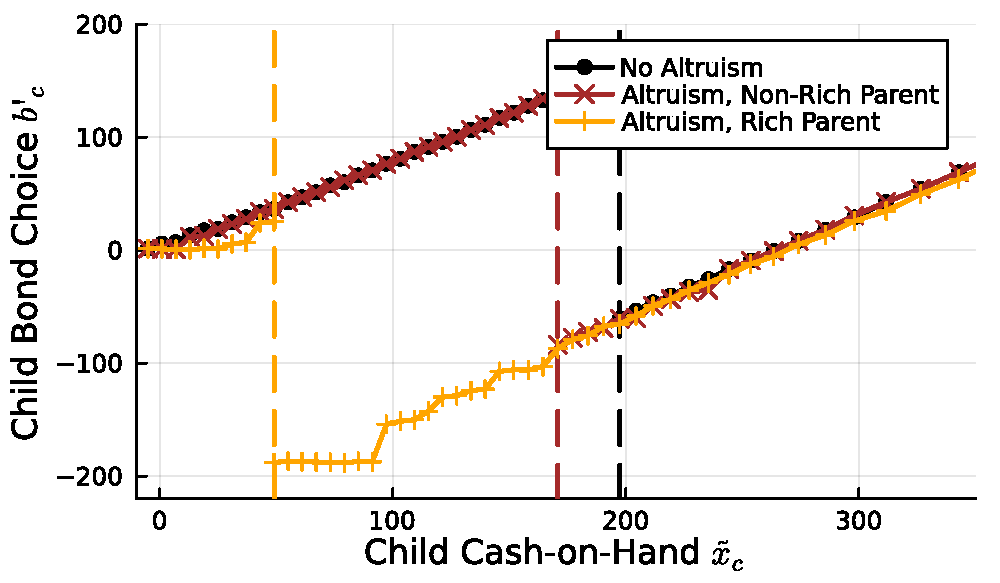
\includegraphics[width=0.6\textwidth]{../tabfig/model/pol_bond.pdf}
	\end{center}
	{\vspace{-0.2in}\begin{footnotesize}\textit{Notes:} The solid lines plots the child’s bond choice ($b'_c$) and the dashed lines the housing choice ($h'_c$) as a function of child cash-on-hand $\tilde x_c$. The dashed vertical lines mark the wealth thresholds at which the child switches from renting to owning. The child states $\mathbf{s}_c'$ are $h'_p$=$h_r$, $y_c$=1.0, $h_c$=$h_o$, and $a_c$=25. The non-rich and rich parent have $b'_p$=100 and $b'_p$=400\unskip. \end{footnotesize}}
\end{figure}

More generally, the child's savings choices show that with altruism, households are more likely to choose to be liquidity constrained, often called hand-to-mouth, as they become homeowners with less wealth and are closer to the borrowing constraints. Altruism reduces the downside of liquidity constraints---namely, the inability to smooth income shocks through partial insurance---while creating the advantage of receiving larger transfers. Given the importance of hand-to-mouth households in aggregate consumption responses \citep[see, e.g.,][]{Kaplan2014a,Boar2020}, this is an important result.

\section{Parameter Selection}\label{sec:estimation}
I estimate the model using data from the PSID and a standard two-step estimation procedure. First, parameters independent of the model structure are estimated from the data or sourced from the literature. Second, I estimate the remaining parameters using simulated method of moments (SMM). I validate the model using nontargeted moments from the PSID as well as experimental evidence from empirical studies. 

For details on the PSID sample selection, see Section \ref{sec:PSID}. Income, wealth, and housing values are winsorized at the 1st and 99th percentiles to control for extreme values. All calculations use family weights. 

\subsection{First Stage: External Parameters}
I report all externally calibrated parameters and their values in Table \ref{tab:calpar}.

\textit{Period Length:} Each period corresponds to two years, matching the PSID interview frequency. I report all parameters in biennial form (e.g., $\beta$ measures how much households discount two years).

\textit{Income Process:} The income process consists of a deterministic life-cycle component $l_a$ for all ages and a persistent shock $y_a$ for children. 

To calibrate the deterministic component, I first find the average income for each age by year and then average over all years. I then regress average income on a fourth-order polynomial of age. The fitted values give the deterministic component for households aged 25 to 65. I find retirement income by dividing the average income for households aged 67 to 83 by the predicted income at age 66 (Figure \ref{fig:y_a}). 

To calibrate the stochastic income process $y_{i,a}$, I first set $N_y=3$ to create a three-state Markov Chain. The sample is divided into age-specific income tertiles. Within each age, I set $v_{i,a}$ as the ratio of the median income for that tertile to the overall median income (Figure \ref{fig:y_ia}). The empirical age-dependent transition matrices provide the transition matrix (Figure \ref{fig:Piv}).

\textit{Housing Parameters:} I set the rental rate $q=0.10$ \citep{Davis2008}, housing depreciation $\delta=0.05$ \citep{Harding2007}, and sales cost $m_s=0.075$ and purchase cost $m_b=0.02$ \citep{Yang2009}. I set the price level to $p=\$232,918/h_o$ to match the average market value of owner-occupied houses for households aged 25 to 44 in my sample. The size $h_o$ is estimated internally.

\textit{Financial Parameters:} Based on \cite{goodman2017sixty}, I set $\overline{PMI}=0.8$ so that households with LTVs above 80\% must pay a PMI premium $r^{PMI}=0.03$. I set $LTV=0.90$, broadly in line with the literature, to account for the mass of loans with LTVs above 80\%. The interest rate on savings is set at $r = 0.04$ (2\% per annum), while the mortgage premium is set at $r^m=0.03$ (1.5\% per annum). Both parameters vary in the literature, but both are typically set around 1\% to 2\% per annum \citep[see e.g.,][]{Cocco2005b,Kaplan2020,Paz-Pardo2019}.
% Mortgage premium: 1 percent in Kaplan et al (0.33 wedge on top of 3% interest rate)
% Mortgage premium: 2 percent in Cocco (2005)
% Mortgage premium: 2 percent in Paz-Pardo

% Risk free rate: 2 percent in Cocco (2005)
% Paz Pardo: 1 + 1 percent in Paz-Pardo
% Kaplan et al 3%

\textit{Risk Aversion, Discount Factor, and Housing Expenditure Share:} I set risk aversion $\gamma=2.0$ and the discount factor $\beta=0.92$ (annualized to $\approx0.96$), standard values in life-cycle models without portfolio choice \citep[see e.g.,][]{Kaplan2020,Boar2018}. The parameter $\xi$ pins down the desired expenditure share of housing consumption and is set to 0.2. This parameter is typically set around 0.15 to 0.25 (e.g., \citealp{Kaplan2020,Chatterjee2015,Paz-Pardo2019,davis2011household}) based on the share of housing expenditures in personal consumption expenditures. Due to minimum house sizes, low-income households generally spend more on rent than implied by $\xi$.
%% ξ parameter:
% Chatterjee 2015: xi=0.15
% Kaplan 2020: xi = 0.16
% Paz Pardo> xi = 0.2
% Vestman (Sweden) xi = = 0.25
% Davis & Ortalo-Magne xi = = 0.24
% Fisher and Gervais (2011) beta = 0.951, gamma = 2.0, 

%% beta:
% Boar 2021 (WP version:) 0.959 (WP version, calibrated to match wealth, risk aversion =2)
% Kaplan 2020: 0.964 (estimated internally, risk aversion =2)
% Paz-Pardo: 0.929 (but have stocks and risk aversion=4)

\textit{Initial Conditions of the Young $y_{c,25},x_{c,25}\sim F(x_{c,53},y_{c,53})$:} 
The initial distribution is set to match the intergenerational correlation in wealth and income. I estimate it nonparametrically for transparency. First, I limit the sample to households aged 24 to 26 with parents 16 to 40 years older. I then divide wealth and income into four and three quantiles, respectively, for both parents and children. The PDF $F(\cdot)$ is then given by the empirical probability of each parent-child combination. The wealth level of a quartile is defined by its median value (Fig. \ref{fig:inidistr})

\newcommand{\parxi}{0.2}
\newcommand{\parbeta}{0.92}
\newcommand{\pargamma}{2.0}
\newcommand{\parq}{0.1}
\newcommand{\pardelta}{0.05}
\newcommand{\parrf}{0.04}
\newcommand{\parrm}{0.03}
\newcommand{\parrpmi}{0.03}
\newcommand{\parPMIlim}{0.78}
\newcommand{\parLTV}{0.9}
\newcommand{\parms}{0.075}
\newcommand{\parmsperc}{8}
\newcommand{\parmb}{0.02}
\newcommand{\parmbperc}{2}
\newcommand{\parprice}{87.96$\times h_o$}
\newcommand{\parhr}{1.0}
\newcommand{\parNdyn}{40000}
\newcommand{\parNgen}{5}
\newcommand{\parnstate}{65}
\newcommand{\parnchoice}{145}
\newcommand{\parNest}{1500}
\newcommand{\parNshrinks}{2}
 
\begin{table}
	\center
	\begin{threeparttable}
		\caption{Summary of Externally and Independently Estimated Parameter}\label{tab:calpar}
		\small
		\begin{tabular}{@{}llll@{}}
    \toprule
    Parameter 			& 		 			& Value  	& Source \\	\midrule
    Period Length		& --				& 2 years   & PSID Frequency \\
    Discount Factor$^\dagger$		& $\beta$			& \parbeta		& Literature (see text)  \\
    Risk Aversion		& $\gamma$			& \pargamma		& Literature (see text)  \\
    Expenditure Share Housing & $\xi$		& \parxi        & Literature (see text) \\
    Rental Price$^\dagger$ 		& $q$				& \parq 		& \cite{Davis2008}  \\
    Deprecation$^\dagger$ 		& $\delta$			& \pardelta		& \cite{Harding2007} \\			
    Risk-free Rate$^\dagger$		& $r^f$ 			& \parrf 	    & Literature (see text) \\
    Mortgage premium$^\dagger$	& $r^m$ 			& \parrm 	    & Literature (see text) \\
    PMI premium$^\dagger$         & $r^{pmi}$         & \parrpmi      & \cite{goodman2017sixty} \\
    PMI limit           & $\overline{PMI}$   & \parPMIlim     & \cite{goodman2017sixty} \\ 
    House Price Level   & $p$		& \parprice      & Data (see text) \\
    Max Loan-to-Value   & LTV 			& \parLTV  & Literature/data (see text) \\
    Selling \& Buying Cost		& ($m_s,m_b$) 			& (\parms,\parmb) &  \cite{Yang2009} \\ 
    Rental Size & $h_r$ & \parhr & Normalization \\
    Deterministic Income & $ l_a$				& Fig. \ref{fig:y_a}		& PSID \\
    Productivity Shocks for Kids & $y,\Pi(y'|y)$ & Fig. \ref{fig:y_ia},\ref{fig:Piv}      & PSID \\
    Initial Distribution & $F(x_{53},v_{53}$)	& Fig. \ref{fig:inidistr}		& PSID \\			
    \bottomrule			
\end{tabular}
		\footnotesize
		\textit{Notes:} Superscript $^\dagger$ denotes parameters that are bi-annualized.
	\end{threeparttable}
\end{table}


\subsection{Moments and Identification}
The remaining three parameters $\theta=\{\eta,\chi,h_o\}$ are estimated internally to minimize the distance between four simulated and empirical moments. 

I estimate the altruism parameter $\eta$ because, relative to previous research, the inclusion of housing introduces new transfer motives, requiring re-estimation to match observed intra-family transfers. Similarly, I estimate the homeownership utility $\chi$, since transfers generate new ownership motives. Finally, I estimate the minimum size of owner-occupied housing, $h_0$, a key parameter in models of homeownership, because housing choices interact with transfer behavior.

\textit{Identification and Moment Estimation:}
I derive all empirical moments from the PSID sample discussed in Section \ref{sec:PSID}. I calculate moments by aggregating over all years, assigning equal weight to each year.

The two most important moments to match are the homeownership and transfer receipt rates of young households, since this is a paper about ownership and transfers. Homeownership pins down the strength of the homeownership utility premium $\chi$ (with a higher premium, more households are homeowners, Fig. \ref{fig:chiid}), while the transfer rate pins down the strength of altruism $\eta$ (with stronger altruism, more households receive transfers, Fig. \ref{fig:etaid}). I exclude transfers below \$500, as they are unimportant for homeownership and including them would increase the transfer rate.

While the model and the PSID have the same two-year frequency, households were asked about transfers in the last calendar year. In my cleaned sample, the annual transfer rate is 24\%. Thus, the two-year transfer rate could range between 24\% and 48\%. To be very conservative, I assume that the two-year transfer rate equals the one-year transfer rate. My estimate of altruism $\eta$ should be viewed as a lower bound.\footnote{I have experimented with targeted higher transfer rates. This requires stronger altruism, which, in turn, increases homeownership motives, lowering the estimated utility premium $\chi$. Overall, the results are qualitatively similar to my conservative estimate, which understates the role of altruistic transfers.}

Finally, I target two moments that govern the selection and timing of ownership---the rent-to-income ratio of renters and wealth at first purchase---to ensure the appropriate selection into homeownership based on income and that marginal first-time owners have the correct wealth levels. The rent-to-income ratio is largely pinned down by the size of the owner-occupied house $h_o$ (larger owner-occupied houses mean that more high-income households rent, reducing the rent-to-income ratio). The wealth at purchase decreases with altruism $\eta$ and the utility premium $\chi$, as they lower the wealth threshold for ownership. For a further discussion of the identification, I refer to Appendix \ref{app:SMM} and Figure \ref{fig:idall}.

\subsection{Model Fit}
I estimate the remaining parameters $\theta=\{\eta,\chi,h_o\}$ as follows. First, let $\hat m$ denote the vector of targeted empirical moments. Given a parameter vector $\theta$, let $\hat m(\theta)$ denote the corresponding model-simulated moments. The estimated parameters minimize the distance between the empirical and simulated moments:
 \begin{equation}
\label{eq:SMM}
 \theta^\star(\Omega) = \arg\min_\theta \left\{[\hat m(\theta) - \hat m]'\Omega [\hat m(\theta) - \hat m]\right\},
\end{equation}
where $\Omega$ is a diagonal weighting matrix with elements equal to the inverse of the squared empirical moments, $1/\hat m^2$. This normalization ensures that no moment receives disproportionate weight due to its units. For details on the estimation procedure, see Appendix \ref{app:SMM}, where I also discuss how the global estimation procedure is used to verify identification and calculate standard errors.

The estimated parameters, reported in Table \ref{tab:esttable}, are consistent with previous literature. The altruism parameter $\eta$ is roughly in the middle of the range in the related literature \cite[see e.g.,][]{Boar2018,Barczyk2020a,Mommaerts2016,Lee2019}. The utility premium of ownership $\chi$ means that the consumption bundle feels about 30\% larger for owners than renters, roughly in line with previous estimates based on life-cycle models \cite[see e.g.,][]{McGee2019,Fisher2011}. The size of the owner-occupied unit relative to the rental is model-dependent, but my estimate falls near the middle of the range in \cite{Kaplan2020}, where the ratio varies from 0.78 to 4.4. The model matches all targeted moments well, though it is overidentified, with no moment being particularly poorly matched. 

%% eta altruism
%Mommaerts 2015: (Limited Commitment) eta = 0.08
% Barczyk 2020a: (0.45)
% Lee & Seshadri: 0.32
% Boar WP: 0.201

%% Extra preference
% Kaplan 2020: 1.015
% Fisher and Gervais 2011: ψy=0.95, ψf=0.87 => \chi = 1/0.95= 1.05 to 1/0.87=1.15
% McGee 1.15

%% House size:
% Kaplan Rentals: {1.17, 1.50, 1.92} owners {1.50, 1.92, 2.46, 3.15, 4.03, 5.15}: Average is 1.98, min,max = (1.5/1.92,5.15/1.17) = (0.78,4.4)
% 

\begin{table}[tb]
	\center 
	\begin{threeparttable}
	\caption{Model Estimation}\label{tab:esttable}
		\begin{tabular}{lrr}
\toprule   
 \textbf{Parameter} & Value & Standard Error\\
\midrule
Altruism ($\eta$) & 0.120 & 0.007\\
Ownership Pref. ($\chi$) & 1.350 & 0.049\\
Size Ratio ($\frac{h_o}{h_r}$) & 2.685 & 0.051\\
\cmidrule(lr){1-3} 

 
\textbf{Moment} & Data & Model\\
\midrule
Owner (25-44) & 0.48 & 0.48\\
Rent / Income (25-44) & 0.23 & 0.23\\
Wealth at Purchase (25-44) & 37.14 & 36.75\\
Transfer Rate (55-74) & 0.24 & 0.24\\
\midrule 
 Sum Squared Distances ($ \times 100$) &  & 0.02\\
\bottomrule
\end{tabular}

	\end{threeparttable}
	{\begin{footnotesize}\begin{flushleft}\vspace{-0.1in}
		\textit{Notes:} Standard errors calculated by estimating the model to 100 bootstrapped empirical samples.
		\end{flushleft}\end{footnotesize}}
\end{table}
\subsubsection{Nontargeted Moments}\label{sec:externalval}
To validate the model, I show that it also matches nontargeted moments. 

First, with a calibrated discount factor of $\beta=0.92$, the model matches the wealth levels of both young and old households. It also replicates the correlation between parental wealth and children's homeownership: in the PSID, young homeowners' parents are 2.5 times wealthier than young renters' parents, compared to about 2 times in the model. This parental wealth gradient effectively captures the intergenerational link in homeownership.

Second, the model aligns well with other moments related to homeownership. It slightly overshoots the age of first homeownership and overpredicts the aggregate homeownership rate of 65\%, primarily due to an excess of homeowner parents stemming from their lack of income risk (see Appendix \ref{sec:robust_incomerisk}). Mortgages are slightly smaller than in the data, as households repay and re-borrow flexibly. The model also matches the LTV ratio for buyers well.\footnote{The empirical LTV is measured at the first observation of ownership, not necessarily at origination, so it can reflect price appreciation, improvements, and mortgage paydown.}

Third, the model also matches transfer-related moments well. It predicts average parental transfers of 2.3\% of parental wealth, close to the 2.6\% estimated from the 2013 Transfer Module (excluding outliers below 0\% or above 100\%). It accurately captures the share of households receiving transfers within two years of house purchases, suggesting proper synchronization of housing transactions and transfers. Renters also receive transfers more often than owners in both the model and the data, though the model slightly overstates this gap.

Fourth, the model fits key dimensions of heterogeneity. It matches the wealth distribution between the 10th and 75th percentiles well, although it slightly overpredicts wealth among the poorest households due to the non-negativity constraint. As with many models, it underpredicts wealth at the top. Finally, it reproduces the positive correlation between income and homeownership across income tertiles, though the model slightly overstates this gap.

\begin{table}
	\begin{adjustbox}{center}
	\begin{threeparttable}
	\caption{Non-Targeted Moments}\label{tab:nontargeted}
	\begin{tabular}{lrr}
\toprule
\multicolumn{1}{l}{Moment} & \multicolumn{1}{c}{Data} & \multicolumn{1}{c}{Model}\\
\midrule
Median Wealth (25-44) & 23.48 & 29.05\\
Median Wealth (55-74) & 189.36 & 211.00\\
Parent Wealth Gradient (med) & 2.60 & 2.04\\
Age First Own (25-44) & 32.45 & 34.15\\
Owner (25-74) & 0.64 & 0.74\\
Mortgage (25-44) & 145.73 & 103.12\\
LTV at Purchase (25-44) & 0.65 & 0.65\\
Transfers / Parental Wealth (55-74) (\%) & 2.59 & 2.60\\
Transfers Around Purchase (25-44) & 0.25 & 0.21\\
Transfers (25-44), Renters & 0.25 & 0.28\\
Transfers (25-44), Owners & 0.22 & 0.18\\
Wealth percentiles, Age 35 (10,25,50,75,90) & -16, 3, 33, 139, 367 & 1, 1, 31, 103, 153  \\ 
Ownership, by income tertile, Age 35 & 0.26, 0.57, 0.79 & 0.26, 0.49, 0.87  \\ 
\bottomrule
\end{tabular}

	\footnotesize 
	\textit{Notes:} Wealth is measured in 1000s of 2016 US dollars.
	\end{threeparttable}
\end{adjustbox}
	\end{table}

\subsubsection{Household-Level Responses to Income Shocks by Parental Wealth}
As a final external validation, I repeat the exercise in Section \ref{sec:eventstudy} (see Figure \ref{fig:housinggrowthrates}), where we saw that households with wealthy parents do not downsize during unemployment spells. Since the model lacks an explicit unemployment state, households are considered unemployed if their productivity drops to the lowest level for a single period. Otherwise, I replicate the exercise exactly. Figure \ref{fig:housinggrowthrates_model} shows that the model matches both the qualitative and quantitative patterns from the empirical data relatively well: Housing consumption falls for households without wealthy parents during ``unemployment,'' while it does not decline for those with rich parents. 

\begin{figure}
	\caption{Event Study: Housing Consumption at Unemployment by Parental Wealth}\label{fig:housinggrowthrates_model}
	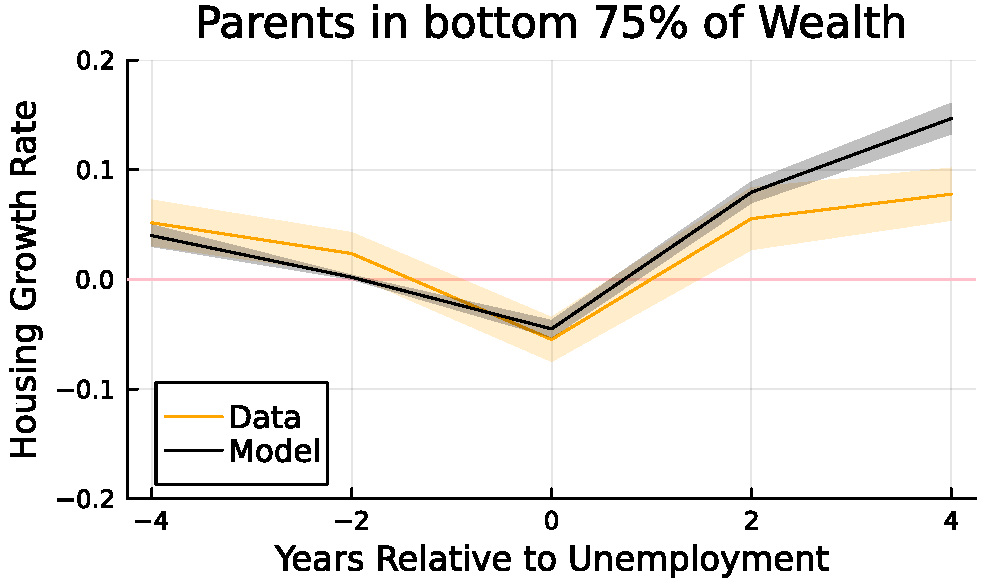
\includegraphics[width=0.5\textwidth]{../tabfig/model_housinggrowthpoor_both}%
	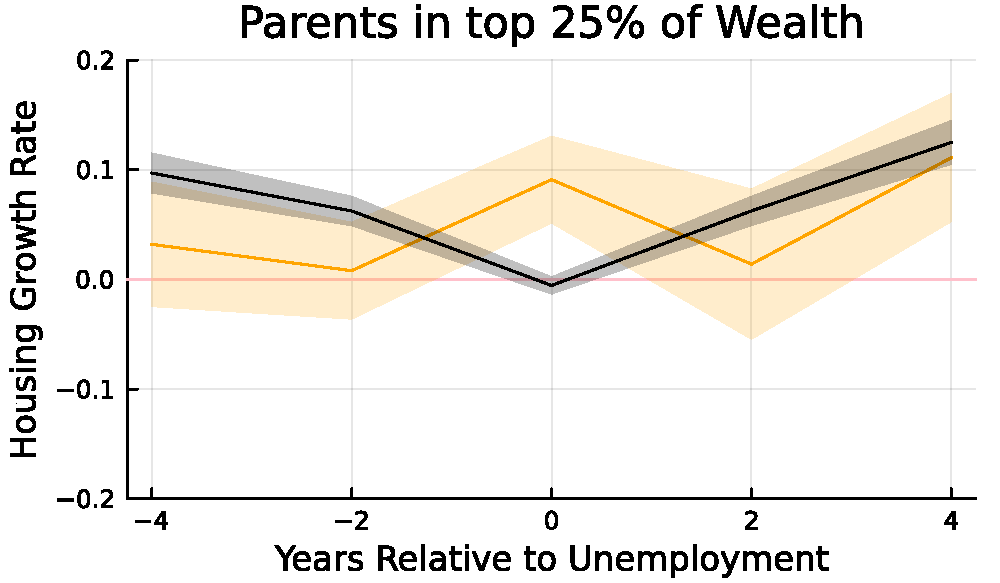
\includegraphics[width=0.5\textwidth]{../tabfig/model_housinggrowthrich_both}
	
	{\begin{footnotesize} \textit{Notes:} Lines denote means, and shaded areas indicate 95\% confidence intervals. The light orange area denotes the empirical estimates (Section \ref{sec:eventstudy}), and the darker grey area denotes the model simulation. The sample consists of households aged 25-45 with exactly one unemployment spell and no changes in head or spouse in the four years before and after unemployment. \end{footnotesize}}
\end{figure}

Taking stock, this section shows that the model can match targeted moments regarding homeownership, transfers, and the transition to homeownership with realistic preference parameter values. The model also matches a set of untargeted moments. Perhaps more importantly, the model replicates the household-level associations between parental wealth and downsizing during income losses. 



\section{Homeownership Rates Without Transfers?}\label{sec:quant}
How important are parental transfers for homeownership? I simulate the model without altruism ($\eta=0$), holding all other parameters constant---the standard model without parent-child interactions.\footnote{Alternatively, I could remove transfers entirely without removing altruism. Since utility is additively separable, the child's choices do not affect the parent's decisions when transfers are absent, aside from a small increase in parental savings due to the intergenerational correlation between wealth and productivity. As this yields nearly identical results, I report only the simpler case of no altruism.} In the main exercise, I assume a perfectly elastic housing supply, meaning that changes in homeownership have no effect on rental or house prices. In Section \ref{sec:endoprice}, I show that the results remain robust even with endogenous housing supply and varying elasticities.

\subsection{The Effect of Parental Transfers on Homeownership}
Table \ref{tab:modelfitnoa} reports how the moments change without altruism and transfers. Homeownership rates decline by 14 percentage points from 49\%, a decrease of 29\% for households aged 25 to 44. This is a large decrease, since households endogenously choose to save more without transfers. By comparison, homeownership only decreased by about 8 percentage points during the financial crisis.

The reduction in homeownership cannot be attributed to an inability to afford buying: Without altruism, median wealth of the young increases (increasing homeownership, in isolation) to the average wealth level at purchase with altruism. The main driver is that the ownership threshold shifts out in wealth without altruism, as we saw in the policy functions (Section \ref{sec:policyfuncs}). Without transfers then, the average wealth at purchase increases by about \$12,500 (about 33\%), the age of first ownership is delayed by about 2.5 years, and the LTV at purchase falls by 13 percentage points. Although homeownership of young households declines sharply, the overall homeownership rate of all households (ages 25 to 74) only falls by 6 percentage points (8\%). Hence, the main aggregate effect of parental transfers is that they induce earlier homeownership. Finally, without altruism, the parental wealth gradient in homeownership decreases from 1.94 to 1.14, with the remaining effect driven by the integenerational correlation in initial wealth and persistent labor productivity.

\begin{table}[tb]
	\center 
	\begin{threeparttable}
		\caption{Homeownership Decreases while Wealth Increases Without Altruism}\label{tab:modelfitnoa}
		\begin{tabular}{lrrr}
\toprule
Moment & Data & \multicolumn{1}{p{2.5cm}}{\centering Altruism \\ $ \eta=0.132 $} & \multicolumn{1}{p{2.5cm}}{\centering No Altruism \\ $ \eta=0 $}\\
\midrule
\textit{Targeted Moments} &  &  & \\
\;Owner (25-44) & 0.49 & 0.49 & 0.35\\
\;Rent / Income (25-44) & 0.23 & 0.23 & 0.22\\
\;Wealth at Purchase (25-44) & 33.09 & 33.20 & 45.78\\
\;Transfer Rate (55-74) & 0.24 & 0.24 & 0.00\\
\textit{Non-Targeted Moments} &  &  & \\
\;Median Wealth (25-44) & 22.89 & 27.64 & 31.67\\
\;Median Wealth (55-74) & 197.08 & 207.75 & 225.09\\
\;Parent Wealth Gradient (med) & 2.61 & 1.94 & 1.14\\
\;Age First Own (25-44) & 32.11 & 33.89 & 36.80\\
\;Owner (25-73) & 0.65 & 0.74 & 0.68\\
\;Mortgage (25-44) & 143.95 & 100.32 & 60.99\\
\;LTV at Purchase (25-44) & 0.66 & 0.66 & 0.53\\
\;Transfers Around Purchase (25-44) & 0.25 & 0.21 & 0.00\\
\bottomrule
\end{tabular}

		\footnotesize
		\textit{Notes:} Wealth is measured in 1000s of 2016 US dollars.
	\end{threeparttable}
\end{table}

\subsubsection{Black-White Homeownership Gap}\label{sec:bwgap}
One natural application of this framework is to quantify how much of the Black-White homeownership gap---young White households are nearly twice as likely to own homes as young Black households---is driven by differences in parental wealth. While existing structural models of racial inequality focus primarily on income and bequests, they typically omit housing and inter-vivos transfers. In contrast, many empirical studies focus on racial difference in housing outcomes.\footnote{For example, \citet{Ashman2020} and \citet{aliprantis2022dynamics} use overlapping-generations models to study the racial wealth gap, attributing most of it to income differences. Though the latter include pooled bequests, they do not model strategic behavior or direct transfers from parents to children. Many empirical studies highlight the role of parental wealth in racial housing gaps: \citet{charles2002transition} find that it explains 25\% of the mortgage application gap,  \citet{bond2021role} attribute 28\% of the gap in maintaining homeownership to parental wealth, and \cite{kermani2021racial} find a large gap in realized housing returns due to distressed sales.}

\begin{table}
	\center
\begin{threeparttable}[tb]
				\singlespacing
		%			\footnotesize
		\caption{Black-White Homeownership Rate}\label{tab:BW_table}
		\begin{tabular}{l rrr rrr}
\toprule & \multicolumn{3}{c}{White} & \multicolumn{3}{c}{Black} \\ \cmidrule(lr){2-4}\cmidrule(lr){5-7}
\multicolumn{1}{c}{Moment} & \multicolumn{1}{c}{Data} & \multicolumn{1}{c}{Altr.} & \multicolumn{1}{c}{No Altr.} & \multicolumn{1}{c}{Data} & \multicolumn{1}{c}{Altr.} & \multicolumn{1}{c}{No Altr.}\\
\midrule
\;Owner (25-44) & 0.53 & 0.52 & 0.39 & 0.26 & 0.24 & 0.22\\
\;Rent / Income (25-44) & 0.22 & 0.22 & 0.21 & 0.25 & 0.27 & 0.27\\
\;Wealth at Purchase (25-44) & 43.69 & 33.76 & 46.52 & 17.17 & 52.05 & 59.25\\
\;Transfer Rate (55-74) & 0.27 & 0.23 & 0.00 & 0.14 & 0.23 & 0.00\\
\bottomrule
\end{tabular}

		\footnotesize
		\textit{Notes:} Wealth is measured in 1000s of 2016 US dollars. See main text for details.
	\end{threeparttable}
\end{table}


I aim to bridge the gap between these structural approaches and empirical results by using my model to quantify the contribution of parental transfers to the Black-White homeownership gap. I repeat the main experiment, seperately for Black and White households, following the methodology in \cite{Ashman2020} and \cite{aliprantis2022dynamics} closely. I shift the income level ($l_a$) according to racial differences: In the matched parent-child household, White households have 8\% higher income and Black households 42\% lower than the average. I then solve the model for White households. For Black households, I reduce house size by 25\% to match observed homeownership rates. I then solve the models both with and without altruism. The results are reported in Table \ref{tab:BW_table}. 

The observed Black-White homeownership gap is $\frac{0.54 - 0.27}{0.54} = 50\%$, compared to 52\% in the model with altruism. Removing altruism reduces the gap to 45\%, implying that parental transfers account for 7 percentage points---or 14\%---of the gap. While Black and White households receive transfers at similar rates in the model, transfers are less influential for Black households, who are further from the ownership threshold and receive smaller amounts. These results highlight the importance of racial differences in parental income, which shape both wealth accumulation and transfer capacity. 

\subsection{Endogenous House Prices}\label{sec:endoprice}
I previously assumed that the supply of homes would fully adjust without affecting prices or rents, reflecting perfectly elastic supply. I now show that the results are similar even when housing supply is endogenous and under different elasticities.

I assume that housing supply ($H^S$) is log-linear in the house price:
\begin{equation}
\label{eq:hsupply}
\ln H^S = \alpha_0 + \alpha_1 \ln p,
\end{equation}
where $\alpha_1$ is the aggregate elasticity of supply to prices. I use a closed-form supply function because the model is too complex to introduce a construction sector. The rent-to-price ratio is unchanged, as in \cite{Kaplan2020}, where rental units are supplied by deep-pocketed landlords who convert rentals to owner-occupied units if the price deviates from the present value of rents. Letting $\alpha_1\to\infty$ yields a perfectly elastic supply function, leaving prices constant, as in the previous section. I first set the elasticity to 3, a typical estimated value for the United States \cite[see e.g.,][]{saiz2010geographic,aastveit2023changing}. Finally, I set the elasticity to 1 as a reasonable lower bound for the long-run aggregate elasticity.

\begin{table}
	\center 
	\begin{threeparttable}
		\caption{Housing Supply Elasticities Not Quantitatively Important}\label{tab:quant_endogenprices}
		
		\begin{tabular}{@{}llll@{}}
			\begin{tabular}{lrrrr}
 \toprule & \multicolumn{1}{c}{Altruism} & \multicolumn{3}{c}{Without Altruism}  \\  \cmidrule(lr){2-2} \cmidrule(lr){3-5} 

Moment & Benchmark & Elastic & Middle & Low\\
\midrule
\textit{Aggregate Moments} &  &  &  & \\
\;Supply Elasticity ($\alpha_1$) &  & $ \infty $ & 3.00 & 1.00\\
\;House Price & 90.66 & 90.66 & 88.65 & 86.64\\
\;Owner (25-73) & 0.73 & 0.68 & 0.69 & 0.70\\
\textit{Targeted Moments} &  &  &  & \\
\;Owner (25-44) & 0.47 & 0.34 & 0.37 & 0.38\\
\;Rent / Income (25-44) & 0.24 & 0.22 & 0.22 & 0.22\\
\;Wealth at Purchase (25-44) & 36.75 & 50.05 & 45.56 & 44.03\\
\;Transfer Rate (55-74) & 0.24 & 0.00 & 0.00 & 0.00\\
\bottomrule
\end{tabular}

		\end{tabular}
		
	\end{threeparttable}
	{\begin{footnotesize}\begin{flushleft}\vspace{-0.1in}%
		\textit{Notes:} I calibrate the housing supply elasticity from equation \eqref{eq:hsupply} as follows. For any elasticity $\alpha_1$, I set $\alpha_0$ to be such that housing supply would equal housing demand in the benchmark model with altruism: $\alpha_0(\alpha_1) = \ln(H^d) - \alpha_1 \ln p$, where $p$ is the benchmark price level (Table \ref{tab:calpar}). The ``Elastic'' column is the same as in the benchmark specification (Table \ref{tab:modelfitnoa}).
	\end{flushleft}\end{footnotesize}}		
\end{table}

Table \ref{tab:quant_endogenprices} reports the results. Allowing house prices to adjust does not meaningfully decrease the contribution of transfers to homeownership or other aggregate outcomes. This is due to the small difference in homeownership rates (ages 25 to 74) with and without altruism. Prices decline by just 7\% even with a supply elasticity as low as 1. Thus, transfers account for between 10 and 13 percentage points of the homeownership rate, depending on the supply elasticity.

\section{Policy Levers, Illiquidity, and MPCs}\label{sec:pol}
I have three main results regarding parental transfers and children's homeownership: (1) how they interact with housing-related policies, (2) how housing illiquidity amplifies their impact, and (3) how they affect marginal propensities to consume (MPCs).

\subsection{Policies and the Importance of Parental Transfers}
Many countries have policies aimed at increasing homeownership, and housing affordability and delayed homeownership is at the forefront of economic policy and research \citep[see e.g.,][]{Mabille2020}. I now evaluate how five different policy levers influence the role of parental wealth in housing outcomes. For each policy, I change the relevant parameter slightly and solve the model before simulating a new distribution. The idea is not to see what the effect of various policy proposals would be in general equilibrium, but how different policy levers interact with parental transfers. The results are reported in Table \ref{tab:policy}. 

\textit{Relaxing Mortgaging Regulation:} To study how parental transfers interact with down payment requirements, I tighten the LTV limit by 3 percentage points. The tighter limit decreases homeownership among the young by 5 percentage points (10\%). Homeownership declines more among households with parents in the middle of the wealth distribution, reducing the parental wealth gradient. While initially counterintuitive, these middle-wealth households rely heavily on small transfers to overcome borrowing constraints; poorer households remain constrained, and richer ones are unaffected. Thus, looser borrowing constraints not only boost homeownership overall but also amplify the importance of parental wealth. Consistent with this mechanism, \citet{wold2024housing} find that owners with poorer parents have lower LTV ratios at origination.

\textit{Lowering PMI:} To study how parental transfers interact with the PMI, which increases the interest rate on high LTV loans, I relax the PMI limit by 7 percentage points. The relaxed PMI limit increases homeownership by 2 percentage points (4\%). Similar to the LTV regulation, homeownership among households with parents in the middle of the wealth distribution rises more, further widening the parental wealth gradient. This result suggests that relaxing the PMI limit increases not only homeownership for all households, but also the role of parental wealth.

\textit{Lowering House Prices:} To study how parental transfers interact with housing affordability, I lower house prices by \$6,000 (7\%). As prices decline, homeownership increases for all households, though more so for households with the richest parents, slightly increasing the role of parental wealth.

\textit{Reducing Purchase Costs:} To study how closing costs and first-time buyer assistance interact with parental transfers, I lower the purchase cost ($m_b$) by 2 percentage points---equivalent to a grant of about \$6,250.\footnote{Many U.S. states offer closing cost assistance to first-time buyers. In England, stamp duty was reduced for first-time buyers in 2017.} While homeownership rises, the gains are concentrated among households with wealthy parents, amplifying the parental wealth gradient. Lowering purchase costs has little effect for renters with non-wealthy parents, who remain constrained by LTV limits and sales costs. In contrast, for household with non-wealthy parents, lower purchase costs reduce the effective price—the main remaining barrier to ownership. This suggests that grants or credits for first-time buyers primarily benefit households of the wealthiest.
 
\textit{Reducing Sales Costs:} 
The earlier empirical results suggested that parental wealth helps offset the illiquidity of housing. To study this interaction, I lower the sales cost $m_s$ from \parms\% to 5. Strikingly, the homeownership rate decreases by 2 percentage points (4\%). This counterintuitive result reflects selection into ownership. homeownership rises slightly among households with the wealthiest and poorest parents but drops sharply---by 9 percentage points---among households with moderately wealthy parents. For these households, lower sales costs weaken the ability to use housing as a commitment device to secure future transfers. In contrast, children of the poorest parents (who rarely receive transfers) and the wealthiest parents (who expect transfers regardless) are less affected.



\begin{table}[tb]
	\centering
	\resizebox{\textwidth}{!}{\begin{threeparttable}
		\caption{Homeownership Policies on the role of Parental Wealth}\label{tab:policy}
		
ratio
		\begin{tabular}{@{}llll@{}}
			\begin{tabular}{l rrrrrr}
\toprule
Moment & \multicolumn{1}{c}{Bench.} & \multicolumn{1}{c}{LTV} & \multicolumn{1}{c}{$PMI$} & \multicolumn{1}{c}{$Price$} & \multicolumn{1}{c}{$m_b$ } & \multicolumn{1}{c}{$m_s$}\\
\; Old Parameter value &  & 0.9 & 0.78 & 90.665 & 0.02 & 0.075 \\ 
\; New Parameter value &  & 0.87 & 0.85 & 88.851 & 0.0 & 0.055 \\ 
\midrule
\textit{Targeted Moments} &  &  &  &  &  & \\
\;Owner (25-44) & 0.47 & 0.44 & 0.51 & 0.50 & 0.52 & 0.45\\
\;Rent / Income (25-44) & 0.24 & 0.23 & 0.24 & 0.23 & 0.24 & 0.24\\
\;Wealth at Purchase (25-44) & 36.75 & 39.11 & 33.99 & 34.52 & 31.76 & 35.94\\
\;Transfer Rate (55-74) & 0.24 & 0.23 & 0.25 & 0.24 & 0.26 & 0.23\\
\textit{By Initial Parent Wealth} &  &  &  &  &  & \\
\;Owner (25-44), Top 33\% & 0.67 & 0.63 & 0.72 & 0.71 & 0.74 & 0.65\\
\;Owner (25-44), Middle 33\% & 0.45 & 0.39 & 0.51 & 0.47 & 0.49 & 0.38\\
\;Owner (25-44), Bottom 33\% & 0.31 & 0.30 & 0.31 & 0.32 & 0.34 & 0.32\\
\bottomrule
\end{tabular}

		\end{tabular}
		
		\footnotesize
			\textit{Notes:} The results are from stationary distributions and ignore transition dynamics. Wealth is measured in 1000s of 2016 US dollars.
	\end{threeparttable}}
\end{table}

These experiments highlight three main findings. First, common policies intended to raise homeownership rates can either strengthen or weaken the role of parental wealth. Relaxing credit constraints increases both homeownership and reliance on parental wealth, as homeownership becomes more attractive to households with wealthier parents. Moreover, in light of the earlier results on the Black–White homeownership gap (Section \ref{sec:bwgap}), broad-based down payment subsidies or tax rebates may unintentionally widen this gap. Second, and in contrast, increasing housing liquidity---by lowering sales costs---reduces the importance of parental wealth. Greater liquidity weakens the role of housing as a commitment device, and can even lower homeownership among children of wealthy parents. 

\subsection{Illiquidity Preference}\label{sec:adjcost}
The previous section established that higher sales costs can increase ownership among households with wealthy parents. Here, I present a more surprising result: Households with wealthy parents prefer illiquidity.

I solve the model both with and without sales costs ($m_s=0$). For each household in the stationary distribution with sales costs, I assess whether they would prefer that neither they nor future generations in their dynasty face sales costs. This hypothetical corresponds to a benevolent agent paying the sales costs for current and future generations in that dynasty only. The results are reported in Table \ref{tab:adjcost}.

Without altruism, all households prefer to remove sales costs. With altruism (baseline calibration), I find that while all parents prefer to remove sales costs, roughly one-quarter of children prefer them. The key determinant is parental wealth: Parents of children who prefer sales costs are approximately three times wealthier. Children who prefer sales costs are also more likely to receive transfers (48\% vs. 13\%) and, conditional on receiving transfers, receive three times larger transfers. Notably, households that own their homes are more likely to prefer sales costs on their housing.

\begin{table}
	\center
	\caption{Household Observables and Support for Keeping Adjustment Cost}\label{tab:adjcost}
	\begin{threeparttable}
		\begin{tabular}{l rrr}
\toprule
  &  \multicolumn{1}{c}{Dislike Costs } & \multicolumn{1}{c}{Prefer Costs } & \multicolumn{1}{c}{All Children}\\
\midrule
Fraction of Children & 0.73 & 0.27 & 1.00\\
Age & 36.21 & 31.65 & 35.00\\
Child Wealth & 35.67 & 24.87 & 29.85\\
Parent Wealth & 128.72 & 410.31 & 183.42\\
Child Ownership Rate & 0.47 & 0.61 & 0.51\\
Transfer Rate & 0.13 & 0.48 & 0.22\\
Transfer Size & 0.66 & 6.45 & 2.20\\
Parents Prefering Costs & 0.00 & 0.00 & 0.00\\
\bottomrule
\end{tabular}

		\footnotesize
		
	\end{threeparttable}
	{\begin{footnotesize}\begin{flushleft}\vspace{-0.1in}%
		\textit{Notes:} Only includes dynasties where the child household is aged 25-44. Wealth is measured in 1000s of 2016 US dollars.
	\end{flushleft}\end{footnotesize}}		
\end{table}

To explore why some households prefer illiquidity, Figure~\ref{fig:prefliq} breaks the sample by liquidity preference and age. Figure~\ref{fig:pref} shows that illiquidity preference declines with age, consistent with reduced reliance on parental transfers; around 50\% of the youngest households prefer illiquidity. The next panels plot homeownership, parental wealth, and child wealth by liquidity preference. Since illiquidity can only be used to extract transfers when the household owns a home and the parent is wealthy, those who prefer it have higher homeownership rates and wealthier parents. Figure~\ref{fig:pref_wealthk} shows that illiquidity-preferring households are initially wealthier, but this reverses around age 33. This flip reflects a tension: to use housing as a commitment device, households must be wealthy enough to own, yet poor enough to remain liquidity-constrained and elicit transfers.

\begin{figure}[tb]
	\captionsetup[subfigure]{aboveskip=-1pt}
	\caption{Liquidity Preference over Age}\label{fig:prefliq}
	\begin{subfigure}{0.5\textwidth}%
		\caption{Prefer Costs}\label{fig:pref}%
		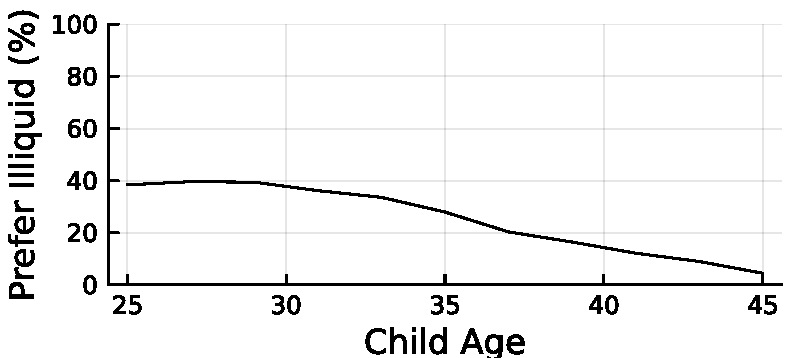
\includegraphics[width=\textwidth]{../tabfig/preferliq/prefer.pdf}%
	\end{subfigure}%
	\hfill
	\begin{subfigure}{0.5\textwidth}%
		\caption{Child's Homeownership}\label{fig:pref_own}%
		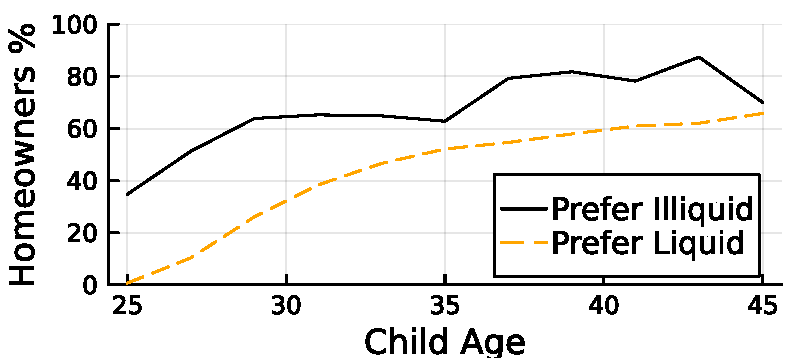
\includegraphics[width=\textwidth]{../tabfig/preferliq/prefer_owner.pdf}%	
	\end{subfigure} 
	\begin{subfigure}{0.5\textwidth}%
		\caption{Parent Wealth}\label{fig:pref_wealthp}%
		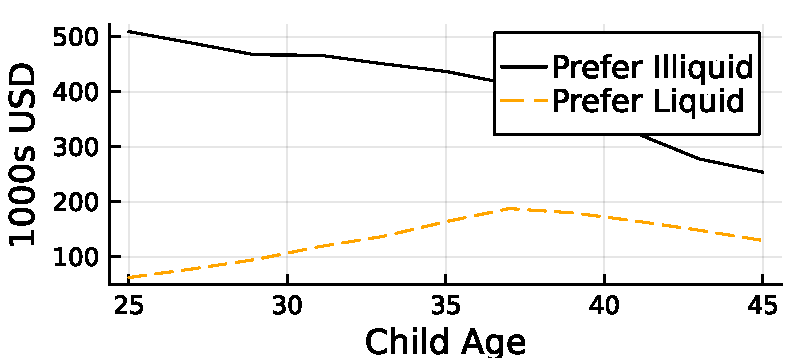
\includegraphics[width=\textwidth]{../tabfig/preferliq/prefer_wealthp.pdf}%
	\end{subfigure}%
	\hfill
	\begin{subfigure}{0.5\textwidth}%
		\caption{Child Wealth}\label{fig:pref_wealthk}%
		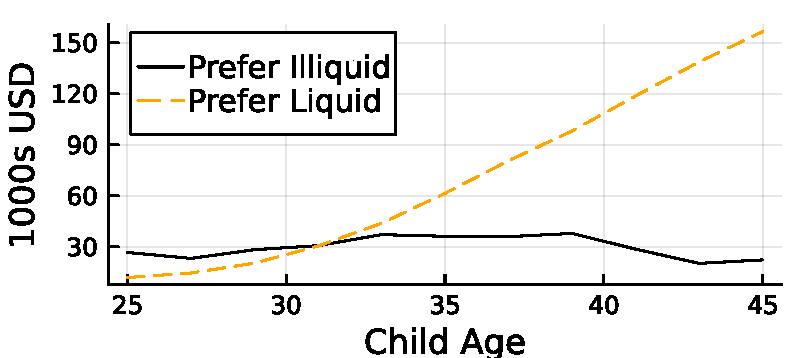
\includegraphics[width=\textwidth]{../tabfig/preferliq/prefer_wealthk.pdf}%	
	\end{subfigure}%
	\caption*{\footnotesize \textit{Notes:} These figures break down the sample of households by whether they prefer illiquidity.}
\end{figure}

In summary, altruism not only reduces the downside of illiquidity but can generate a preference for it. As in models of behavioral biases, households use housing illiquidity as a commitment device to keep marginal utility high in the future. With altruism, this induces transfers; with time inconsistency, it promotes saving \citep{attanasio2024temptation}. 

\subsection{MPCs}
If altruism makes illiquid assets more attractive, a natural question is how altruism affects MPCs, as liquidity constraints are an important driver of MPCs \citep[see e.g.,][]{aguiar2024hand,Kaplan2014,fagereng2021mpc}. We begin by computing counterfactual MPCs for households in the stationary distribution, assuming no altruistic transfers. The average MPC of young households is 0.35. The MPC of liquidity constrained households (0.44) is about three times that of unconstrained households (0.16). While these MPCs are lower than empirical estimates---typically ranging from 0.5 to 0.9---they are relatively standard in models not designed to generate high MPCs. 

Introducing altruistic transfers generates two offsetting effects. First, future transfers increase MPCs by decreasing precautionary savings motives. This effect is small, and only increases the average MPC by about 3 percentage points. The increase is almost entirely driven by unconstrained households. Second, current transfers provide partial insurance and decrease MPCs. This effect is large, reducing the MPC by 11 percentage points. The decrease is almost entirely driven by liquidity constrained households. Finally, altruism---including current and future transers---reduces the MPC from 0.35 to 0.25. Altruistic transfers lower the MPC of liquidity constrained households but increases it for unconstrained households---the ratio of MPC for liquidity constrained to unconstrained decreases from 3 to 2.


\begin{table}[tb]
	\center\singlespacing	
	\begin{threeparttable}[tb]
		\caption{Altruistic Transfers Decrease the MPC}
		\begin{tabular}{lrrr}
\toprule
  & \multicolumn{1}{c}{Mean} & \multicolumn{1}{c}{Liq. Constrained} & \multicolumn{1}{c}{Liq. Unconstrained} \\
\midrule
No Altruism & 0.35 & 0.45 & 0.16\\
\;Future transfers only & 0.38 & 0.47 & 0.21\\
\;Current transfer only & 0.24 & 0.30 & 0.13\\
Altruism & 0.25 & 0.31 & 0.15\\
\bottomrule
\end{tabular}

	\end{threeparttable}
	{\begin{footnotesize}\begin{flushleft}\vspace{-0.1in}
		\textit{Notes:} Sample includes all households aged 25-44 in the stationary distribution. Following \cite{Kaplan2014}, households are liquidity constrained if they have negative liquid wealth $(b_k)$ exceeding 16.5\% of annual earnings. The MPC is calculated from a \$5,000 positive shock.\end{flushleft}\end{footnotesize}}			
\end{table}

These results have several implications for the MPC literature. First, model-implied MPCs may be overstated when informal intra-family transfers are omitted, particularly for households with wealthy parents. Second, a common strategy to match high MPCs is to introduce households with low target wealth—e.g., through impatience \citep{aguiar2024hand}—but such behavior is observationally similar to that of households expecting altruistic support. Third, models that generate high MPCs by introducing illiquid assets with large return premia \citep{kaplan2022marginal} may overlook the fact that homeowners with wealthy parents have access to informal insurance, which lowers their effective MPC. 

\section{Conclusion}
In this paper, I demonstrate that parental transfers play a large role in households' homeownership decisions. I build and estimate a dynamic life-cycle model of homeownership where altruistic parents may transfer to their adult children in every period. I use the model to quantify the importance of parental transfers for young adults' homeownership and to understand how policies that lower barriers to homeownership interact with these transfers.

Using a counterfactual experiment without altruism (a standard life-cycle model), I find that transfers account for 14 percentage points (29\%) of the homeownership rate. I show that policies that lower entry barriers to homeownership amplify the importance of parental wealth on housing outcomes, while those that lower the downsides of illiquid homeownership reduce the importance of parental wealth. Finally, I study the role of housing illiquidity and parental transfers. My paper thus contributes to a better understanding of the determinants of homeownership and to the growing literature on the role of family economics in shaping macroeconomic outcomes (e.g., \cite{Doepke2016a,Daruich2018}).

Another contribution of the paper is to include an illiquid asset in the altruism framework. With altruistic parents, transfers generally flow to borrowing-constrained households, since they have a large marginal utility of wealth \citep{Barczyk2020,Chu2020}. With a single asset, this framework implies that households who receive transfers are poor. In the data, around 20\% of all households are ``wealthy hand-to-mouth'' and have positive wealth but no liquid wealth \citep{Kaplan2014a,Attanasio2018}. My paper bridges these two strands of the literature. First, I show that some households with wealthy parents choose to be liquidity-constrained to receive larger transfers. While it is difficult to test this prediction, my empirical results are consistent with this behavior: parental wealth improves housing outcomes after purchase, including ownership retention, lower delinquency, and less downsizing in unemployment. Second, I show that the lack of commitment generates preferences for illiquidity, even when households are rational and without behavioral biases \citep[see e.g.,][]{attanasio2024temptation}. 

I made several simplifying assumptions to keep the model tractable. Adding richer housing dynamics and equilibrium effects would allow one to study other interesting questions, such as the extent to which transfers contribute to house price growth. My model omits a feedback loop, in which transfers raise demand and, thus, house prices, boosting the wealth of homeowning parents and, thus, higher transfers, and so on. Another potential extension could examine whether illiquidity may reduce the commitment problem in the family. Additionally, my preferences-for-illiquidity results have implications for the literature on high-MPC households \citep[see e.g.,][]{kaplan2022marginal}. In particular, we are likely overestimating the average MPC of liquidity-constrained households with wealthy parents, since these households use parental transfers to smooth shocks. For example, following a negative shock, consumption may fall less due to transfers, while for positive shocks, consumption may rise less as parents reduce transfers.

\newpage
\begingroup\singlespacing
\bibliographystyle{ecta}
\bibliography{bibliography}
\endgroup
\newpage


\appendix

\setcounter{figure}{0}
\renewcommand{\thefigure}{A\arabic{figure}}
\setcounter{table}{0}
\renewcommand{\thetable}{A\arabic{table}}

\section{Transfers and the Rent-to-Own Transition}\label{app:rent_to_own}
A large literature documents that parental transfers increase the probability that renters become homeowners (e.g., \citealp{wold2024housing}; \citealp{Blickle2019}; \citealp{benetton2022dynastic}; \citealp{Guiso2002}; \citealp{Engelhardt1998}), I replicate this result to highlight the importance of transfers for housing outcomes. 

I estimate
\begin{equation}	\label{eq:transferrent}
	\Pr\left(Own_{i,t+2}=1 \mid Own_{i,t}=0\right)
	= \alpha + \beta\,Transfer_{i,t+2}
	  + \gamma' X_{i,t} + \varepsilon_{i,t},
\end{equation}
where \(Own_{i,t}=0\) denotes renting at time \(t\), \(Transfer_{i,t}=1\) if the household received a transfer between survey waves, and \(X_{i,t}\) includes log parental wealth, log household income, log household net worth, log household size, age, parental age, and dummies for  education, marital status, race, household composition changes, and state and year fixed effects. The sample is limited to renting households aged 25 to 44 who have never been observed as homeowners. Table \ref{tab:newowners} reports the estimated coefficients. These regressions are similar to those in \cite{Lee2018}, who also use the PSID.  It is important to note that transfer receipt is not exogenous---many transfers may be made precisely because the renter is buying a home.

I use two definitions of transfer receipt. The narrow definition includes parental gifts over \$500 in 2012, limiting the sample to renters in 2011. The broad definition includes any gift or inheritance over \$10,000 reported in any wave, or a large parental gift in 2012. This allows for household fixed effects and a larger sample, but captures only large transfers and includes some non-parental ones.

In a univariate regression, receiving a parental transfer is associated with a 2.9 percentage point higher probability of becoming a homeowner in 2013 among renters in 2011. With a full set of controls parental transfers are associated with a 1.2 percentage point higher probability of becoming a homeowner. This represents a substantial increase relative to the baseline rent-to-own transition rate of about 14\%, though the effect is not statistically significant. 

To increase statistical power, I now use the broader transfer definition, which includes all large transfers. This expands the sample size tenfold but reduces the transfer receipt rate to around 3\%, while the median transfer size rises from \$1,500 to \$24,200. The broader sample also allows me to follow renters over time and include household fixed effects. In a univariate regression, transfer receipt is associated with a 21.9 percentage point increase in the probability of becoming a homeowner. Even with a full set of controls, the effect remains large and statistically significant: 13.5 percentage points in the OLS specification ($p<0.001$) and 7.9 percentage points with household fixed effects ($p<0.1$). These magnitudes are substantial compared to the baseline rent-to-own transition rate of 18\%.

\begin{table}
	\center
	\begin{threeparttable}
		\caption{The Transition to Ownership}
		\label{tab:newowners}
		\small 
				{
\def\sym#1{\ifmmode^{#1}\else\(^{#1}\)\fi}
\begin{tabular}{l*{5}{c}}
\toprule
                &\multicolumn{1}{c}{(1)}&\multicolumn{1}{c}{(2)}&\multicolumn{1}{c}{(3)}&\multicolumn{1}{c}{(4)}&\multicolumn{1}{c}{(5)}\\
                &\multicolumn{1}{c}{OLS}&\multicolumn{1}{c}{OLS}&\multicolumn{1}{c}{OLS}&\multicolumn{1}{c}{OLS}&\multicolumn{1}{c}{FE}\\
\midrule
\textit{Transfer}&                  &                  &                  &                  &                  \\
\;Parent Transfer&    0.016         &                  &                  &                  &                  \\
                &  (0.041)         &                  &                  &                  &                  \\
\;Any Transfer  &                  &    0.032         &                  &                  &                  \\
                &                  &  (0.040)         &                  &                  &                  \\
\;Any Transfer ($>$10k)&                  &                  &    0.077         &    0.136\sym{***}&    0.086\sym{*}  \\
                &                  &                  &  (0.092)         &  (0.032)         &  (0.042)         \\
\textit{Other Controls}&                  &                  &                  &                  &                  \\
\;Par. Wealth   &    0.000         &   -0.001         &   -0.001         &    0.001         &    0.005         \\
                &  (0.013)         &  (0.013)         &  (0.013)         &  (0.004)         &  (0.006)         \\
\;Net Worth     &    0.041\sym{***}&    0.041\sym{***}&    0.040\sym{***}&    0.020\sym{***}&    0.010\sym{**} \\
                &  (0.011)         &  (0.011)         &  (0.012)         &  (0.003)         &  (0.004)         \\
\;Income        &    0.034         &    0.034         &    0.034         &    0.049\sym{***}&    0.013         \\
                &  (0.023)         &  (0.023)         &  (0.023)         &  (0.007)         &  (0.009)         \\
\;High School=1 &   -0.028         &   -0.027         &   -0.026         &    0.029\sym{*}  &   -0.025         \\
                &  (0.038)         &  (0.039)         &  (0.038)         &  (0.011)         &  (0.035)         \\
\;College=1     &    0.077         &    0.078         &    0.082         &    0.084\sym{***}&    0.100\sym{+}  \\
                &  (0.055)         &  (0.056)         &  (0.055)         &  (0.018)         &  (0.061)         \\
\;Married=1     &    0.021         &    0.021         &    0.021         &    0.091\sym{***}&    0.040         \\
                &  (0.037)         &  (0.037)         &  (0.037)         &  (0.013)         &  (0.030)         \\
\;White=1       &    0.003         &    0.002         &    0.001         &    0.048\sym{***}&    0.191\sym{*}  \\
                &  (0.038)         &  (0.038)         &  (0.038)         &  (0.012)         &  (0.091)         \\
\;Family Size   &   -0.007         &   -0.008         &   -0.007         &   -0.016         &    0.011         \\
                &  (0.027)         &  (0.027)         &  (0.027)         &  (0.010)         &  (0.020)         \\
\midrule
N               &      635         &      633         &      633         &    6,925         &    6,925         \\
Receipt Rate    &    0.194         &    0.215         &    0.055         &    0.035         &    0.035         \\
Rent-to-Own Rate&    0.139         &    0.139         &    0.139         &    0.181         &    0.181         \\
\bottomrule
\end{tabular}
}


		{\begin{footnotesize}\begin{flushleft}
		\textit{Notes:} Standard errors in parentheses, clustered at the household level. \textsuperscript{+}$p<0.10$, \textsuperscript{*}$p<0.05$, \textsuperscript{**}$p<0.01$, \textsuperscript{***}$p<0.001$.
		\end{flushleft}\end{footnotesize}}		
	\end{threeparttable}
\end{table}


\section{Quantitative Model Details} 

\subsection{Decision Problems at Age 53 and 83}\label{sec:decextra}
As depicted in Figure \ref{fig:overview}, several transitions occur between age 53 and 55: The `old' parent dies, the `old' child becomes a `new' parent, and the `new' child becomes economically active. 

These transitions mean that the child's decision problem at age 53 is very different from earlier ages (Eq. \ref{eq:Vk}). First, the continuation value is now the parent's value function at age 25 of the new child ($V_{p}({\mathbf{s}'_{p,25}})$). Second, the expectation is over the new child's initial productivity and net worth ($x_{c,25},v_{c,25}\sim F(x_{c,53},y_{c,53}$)), instead of the old child's productivity. Third, the law of motion now includes bequests from the old parent instead of a transfer. Fourth, it is necessary to map next-period variables for the old child into variables for the new parent. The problem, for a child aged 53 who choose to own, becomes:
\begin{equation*}
\begin{split}
V_c(\mathbf{s}_{c,53;\mathbf{g}_p})^{own} = &\max_{c_{c,53},b'_{c,53},h'_{c,53}=h_o} u(c_{c,53},h'_{c,53}) + \beta \E_{y_c}\left[V_{p}({\mathbf{s}'_{p,25}};\mathbf{g_c}) \right] \\
\text{s.t.}\quad & 	b'_{c,53} = \tilde x_{c,53} - c_{c,53} - p h'_{c,53}  - m_b p h'_{c,53} \\
& x'_{p,25} = b'_{c,53}(1+r(b'_{c,53})) + x'_{p,53} \\
& b'_{c,53} \ge -LTV p h'_{c,53}, \\
& h_{p,25} = h'_{c,53},
\end{split}
\end{equation*} 
where $c,53$ and $p,53$ denote the variables associated with old child and old parent in this period, and $c,25$ and $p,25$ denote the variables associated with the new child and new parent in the next period. The last equation maps the old child's housing choice into the new parent's---the same household one period later---housing state. The same mapping applies to the law of motion (third equation).

The dying parent's decision problem undergoes similar changes (Eq. \ref{eq:Vp}). First, the continuation value is now the new parent's value function at age 25 of the new child, weighted by altruism ($\eta V_p(\mathbf{s}'_{p,25})$). The remaining changes---namely the expectation, the law of motion, and the mapping of next-period variables---are the same as for the child, and thus the decision problem is modified in the same way.

\begin{equation*}
	\begin{split}
	V_p(\mathbf{s}_{c,53};\mathbf{g}_c)^{own} = &\max_{c_{p,53},b'_{p,53},h'_{p,53}=h_r} u(c_{p,53},h'_{p,53}) + \eta u(c_{c,53},h'_{c,53}) + \beta \eta \E_{y_c}\left[V_{p}({\mathbf{s}'_{p,25}},\mathbf{g}_p) \right] \\
	\text{s.t.}\quad & b'_{p,25} = x_{p,53} + w_{p,53} - c_{p,53} - t_{p,53} - q p h_{p,53}'\\
	& x_{p,53}' = b'_{p,53}(1+r(b'_{p,53})) \\
	& t_{p,53}\ge0, \\
	& b'_{p,53}\ge 0. \\
	\end{split}
\end{equation*} 


\subsection{Measures of Households}\label{sec:hhmeasures}
The state-space of a parent is $S_p = X_c \times X_p \times Y_c \times H_c \times H_p \times A_c$, with $\mathbf{s}_p$ denoting generic elements therein and $\mc{S}_p$ the associated Borel-$\sigma$ algebra. The state space of a child is $S_c= B_p \times H_p \times X_c \times Y_c \times H_c \times A_c$, where $B_p=\mathbb{R}$. For conciseness, I omit further definitions for the child. Let $\psi_p(\mathbf s_p)$ be a probability measure over $(S_p,\mc{S}_p)$ so that $\psi(\mathbf s_p)$ denotes the measure of households with state $\mathbf s_p$ (i.e., after the shock is realized but before choices are made). Finally, $\Psi_p$ denotes the corresponding cumulative distribution function. The mass of households for each age is normalized to 1/15.

\textit{Law of Motion for Dynasties with Children Aged 25-51:} The mass of households in state $\mathbf{s}_p$ is the mass of families adopting housing and savings policies that lead them to this state, adjusted by the probability of experiencing a given income shock:
\begin{equation}\label{eq:LoM}
\begin{split}
\psi(\mathbf{s}'_p) = \int_{\mathbf{s}_p\in \mathcal{S}_p} & 
\mathbf{1}_{\left\{ x'_p = x'^*_p(\mathbf s_p) \right\} }
\mathbf{1}_{\left\{ h'_p = h'^*_p(\mathbf s_p) \right\} } 
\mathbf{1}_{\left\{ x'_c = x'^*_c(\mathbf s_c(\mathbf s_p))\right\}} 
\mathbf{1}_{\left\{ h'_c = h'^*_c(\mathbf s_c(\mathbf s_p))\right\}} \times \\
&\pi(y'_c|y_c)\diff \psi(\mathbf s_p).
\end{split}
\end{equation}
Note that the child's state $\mathbf{s}_c(\mathbf{s}_p)$ in these expressions depend on the choices of the parent which depend on their state. For example, 
\begin{equation}
h'^*_c\left(\mathbf s_c(\mathbf s_p)\right) =h'^*_c\left(b_p'^*(\mathbf{s}_p),h_p'^*(\mathbf{s}_p'),x'_c + t_p'^*(\mathbf{s}_p'),y'_c,h_c',a_c+2 \right).
\end{equation}

\textit{Law of Motion for Children Aged 53:} In this special case, the distribution will depend on the choices of the new parent (old child), the now deceased parent and the stochastic initial conditions of the new child. 
\begin{equation}\label{eq:LoM55}
\begin{split}
\psi(\mathbf{s}'_p;a_c=25) = \int_{\mathbf{s}_p\in \mathcal{S}_p} & 
\mathbf{1}_{\left\{ x'_p = x^*_p(\mathbf s_p) + x^*_c(\mathbf s_c(\mathbf s_p)) \right\} }
\mathbf{1}_{\left\{ h'_p = h^*_p(\mathbf s_p) \right\} } 
\mathbf{1}_{\left\{ h_c' = h_r\right\}} \times \\
&F(x_c',y_c'|x_c,y_c) \diff \psi(\mathbf s_p;a_c=53),
\end{split}
\end{equation}
where we limit $s_p$ to only include the subset of the state-space where $a_c=53$. The initial wealth and productivity of the child depends on the wealth $x_c$ and productivity $y_c$ of the new parent at age 53. Further, all children start out as renters, and the next-period wealth of the new parent is savings plus bequests.

Finally, the function $\mathcal{H}$ operates on the distribution $\psi(\mathbf{s}_p)$ and policy functions %$g^*(\mathbf{s}_p):\mathbf{S}_p \rightarrow (X\times B \times T \times H)\times (X\times B \times H) \times (A_c)$ 
and maps them into a new distribution in accordance with equations (\ref{eq:LoM}, \ref{eq:LoM55}):
\begin{equation}\label{eq:DisIter}
\psi_{n+1} = \mathcal{H}(\psi_n,g^*),
\end{equation}
where the subscript denotes the iteration of the distribution. A stationary distribution is then a fixed point of equation \ref{eq:DisIter}.


\section{Estimation}\label{app:SMM}
In the internal estimation, I first draw $N=\parNest$ 3-dimensional candidate parameter vectors $\theta$, using Sobol sequencing. I then rank the vectors by the objective function, and use the top 5\% to set the bounds of a new Sobol sequence, from which I draw another {\parNest} candidate parameter vectors. I shrink the search space {\parNshrinks} times. 

The global optimization procedure facilitates verifying identification. First, pick a parameter, say $h_o$, and divide it into 20 quantiles. The remaining parameters are uniformly distributed within each quantile. Next, find the 25th, 50th, and 75th percentiles within each quantile for a moment. We can then plot how the moment depends on the parameter by plotting the percentiles over quantiles. A moment is informative for a parameter if the percentiles shift as we move across the parameter's quantiles. A steeper slope indicates a more informative moment for the parameter. A parameter is relatively more important when the spread between the 25th and 75th percentiles is smaller. 

The results of this exercise are plotted in Figure \ref{fig:idall}. For example, take the house size $h_o$ (Fig. \ref{fig:hoid}), where we see that the rent-to-income ratio decreases with the size of owner-occupied housing. The tightness of the 25th and 75th percentiles indicates that the other parameters have little effect on the rent-to-income ratio. The other moments are not sensitive to the house size. Finally, I also plot the SMM objective function (Eq. \ref{eq:SMM}) over $\eta$, showing that the global search space is wide enough. The results for the remaining parameters are shown in the other panels of Figure \ref{fig:idall}.

\begin{figure}\caption{Identification of $\eta,h_0,\chi$.}\label{fig:idall}
	\begin{subfigure}{\textwidth}\caption{Identification of $h_o$}\label{fig:hoid}
		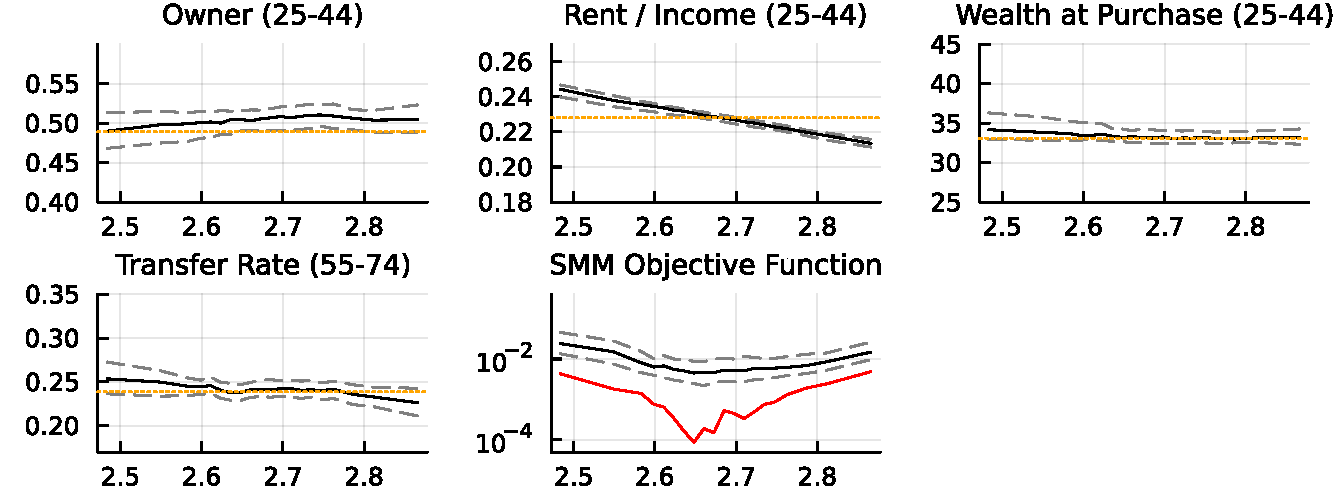
\includegraphics[width=\textwidth]{../tabfig/est/identification/ho.pdf}
	\end{subfigure}
	\begin{subfigure}{\textwidth}\caption{Identification of $\eta$}\label{fig:etaid}
		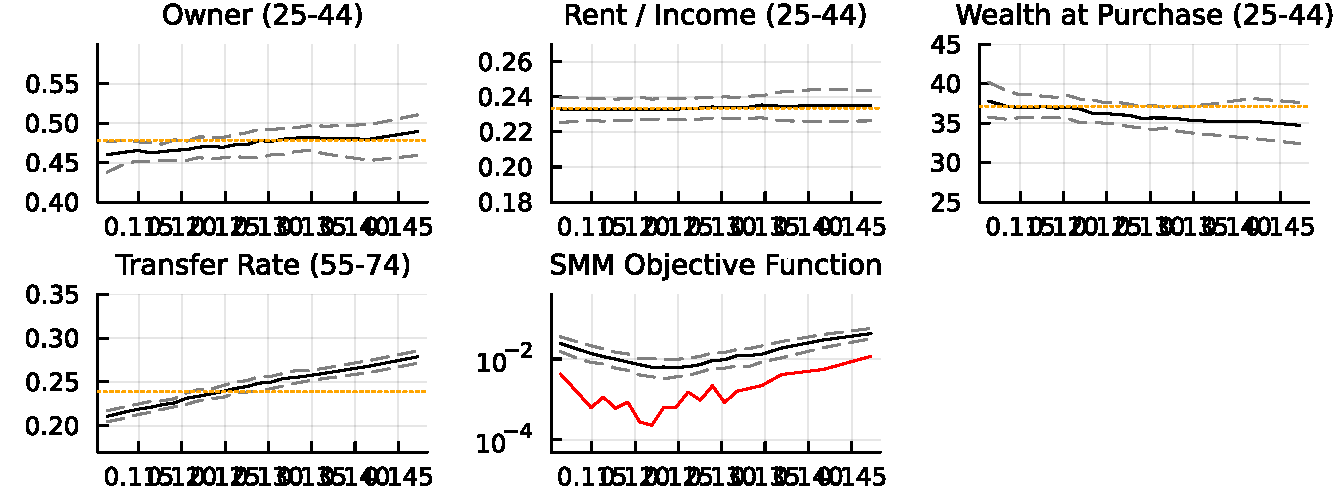
\includegraphics[width=\textwidth]{../tabfig/est/identification/eta.pdf}
	\end{subfigure}
	\begin{subfigure}{\textwidth}\caption{Identification of $\chi$}\label{fig:chiid}
		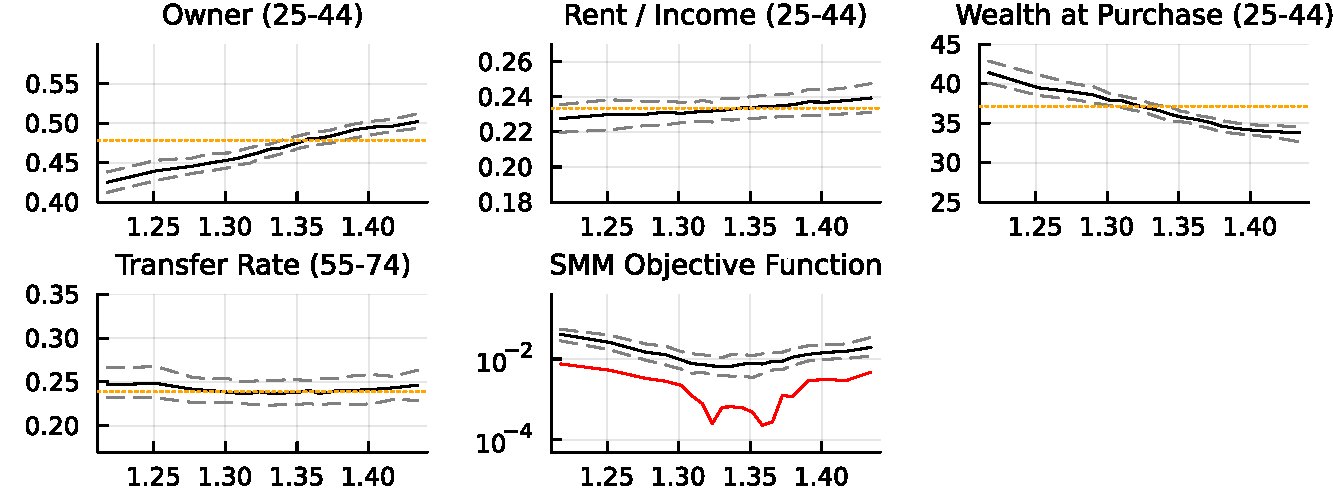
\includegraphics[width=\textwidth]{../tabfig/est/identification/chi.pdf}
	\end{subfigure}
	{\begin{footnotesize} \textit{Notes:} Dashed grey lines denote the 25th and 75th percentiles, the solid black line the median, the solid red line the minimum (only used for the SMM objective function value), and the dashed orange horizontal line the empirical moment (not applicable for the SMM objective function).\end{footnotesize}}
\end{figure}


\section{Robustness Exercises}
\subsection{Parental Income Risk}\label{sec:robust_incomerisk}
In the benchmark model, households face no income risk after age 55. I now show that the results are robust to this assumption. To do so, I perform the following modifications. First, the labor income of parents is now assumed to be the product of a transitory productivity shock:
\begin{equation*}
w_{i,a} = l_a \nu_{i,a} \; \forall a\in\{55,57,\dots,83\}. \label{eq:wp2}
\end{equation*}
The process is calibrated as follows. First, I keep households aged 55-85. I subtract healthcare expenditures from household income as healthcare expenditure risk is a significant risk for older households \citep{denardi2024}. Next, I divide the sample into year-age specific income tertiles, find the median income within each age, and average over years to find the parent productivity shifter $\nu_{i,a}$. The results, fitted to a cubic trend, are plotted in Figure \ref{fig:nu}. The shock is transitory, and the PDF $\Pi(\nu)$ takes the value 1/3 for any outcome.

The results are reported in Table \ref{tab:robust}. We see that the introduction of income risk for the old has neglible effects and leaves the main findings intact. Income risk for parents lower their homeownership rate a touch while increasing their wealth a wee bit. Parental transfers still account for 14 percentange points of the homeownership rate of young households.

\subsection{Aggregate Price Risk}\label{sec:robust_pricerisk}
In the benchmark model house prices are certain. I now show that the results are robust to introducing price risk in the manner of \cite{Corbae2015}. This introduces a new state variable $z$ that denotes the aggregate price level, and the house price is either low, normal, or high depending on the value of $z$. The transition matrix for $z$ follows 
\begin{equation}
\Pi(z'|z) = \begin{bmatrix}
0.90 & 0.10 & 0.00 \\
0.02 & 0.96 & 0.02 \\
0.00 & 0.25 & 0.75 \\
\end{bmatrix}.
\end{equation}
The aggregate house prices are set to be $(p_l,p_n,p_h)=(0.7,1.0,1.3)p_{bench}$, where $p_{bench}$ is set to be the estimated value from Table \ref{tab:esttable}. I then solve the model with price uncertainty, but simulate the economy when house prices are at the normal level. 

The results are reported in Table \ref{tab:robust}. We see that the introduction of aggregate price uncertainty increases savings for old households, with and without altruism. It also induces households to buy housing slightly later, with lower LTV's and higher wealth at purchase. However, the main quantitative finding remains: Parental transfers now account for 11pp (25\%) of the homeownership rate. I have also perform robustness checks where I allow for transitory idiosyncratic dividend/return shocks as in \cite{Chang2024} for homeowners, and find that, as expected, idiosyncratic price risk have even smaller quantitative effects.



\begin{figure}
    \caption{Calibration of Parental Income Shocks}\label{fig:nu}
	{\centering
    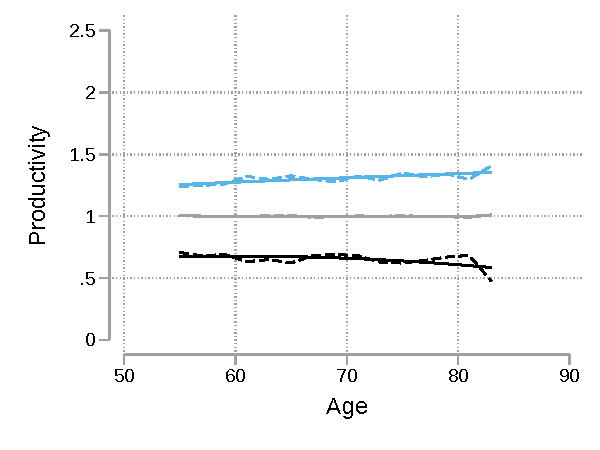
\includegraphics[width=0.5\textwidth]{../tabfig/empirical/lifecycleproductivity_old_3}
    \par}    {\begin{footnotesize} \textit{Notes:}
        Dashed lines are the empirical age-medians, and solid lines are fitted second-order polynomials used in model calibration. The lines denote the value of $\nu_{i,a}$ in the first tertile (black), middle (gray), and top (blue) by age.
    \end{footnotesize}}
\end{figure}


\begin{table}
	\center 
	\resizebox{\textwidth}{!}{
	\begin{threeparttable}
		\caption{Results Robust to Old-Age Risk and Uncertain House Prices}\label{tab:robust}
		\begin{tabular}{lr rr rr rr}
 \toprule & & \multicolumn{2}{c}{Benchmark} & \multicolumn{2}{c}{Old Risk} & \multicolumn{2}{c}{Price Risk}
 \\  \cmidrule(lr){3-4}\cmidrule(lr){5-6}\cmidrule(lr){7-8}
Moment & Data & \multicolumn{1}{c}{$ \eta>0 $} & \multicolumn{1}{c}{$ \eta=0 $} & \multicolumn{1}{c}{$ \eta>0 $} & \multicolumn{1}{c}{$ \eta=0 $} & \multicolumn{1}{c}{$ \eta>0 $} & \multicolumn{1}{c}{$ \eta=0 $}\\
\midrule
\textit{Targeted Moments} &  &  &  &  &  &  & \\
\;Owner (25-44) & 0.49 & 0.49 & 0.35 & 0.49 & 0.35 & 0.45 & 0.34\\
\;Rent / Income (25-44) & 0.23 & 0.23 & 0.22 & 0.23 & 0.22 & 0.22 & 0.21\\
\;Wealth at Purchase (25-44) & 33.09 & 33.20 & 45.78 & 35.64 & 45.83 & 34.91 & 50.30\\
\;Transfer Rate (55-74) & 0.24 & 0.24 & 0.00 & 0.24 & 0.00 & 0.21 & 0.00\\
\textit{Non-Targeted Moments} &  &  &  &  &  &  & \\
\;Median Wealth (25-44) & 22.89 & 27.64 & 31.67 & 28.89 & 31.68 & 27.68 & 31.67\\
\;Median Wealth (55-74) & 197.08 & 207.75 & 225.09 & 212.72 & 229.21 & 213.50 & 218.36\\
\;Parent Wealth Gradient (med) & 2.61 & 1.94 & 1.14 & 1.66 & 1.12 & 1.71 & 1.12\\
\;Age First Own (25-44) & 32.11 & 33.89 & 36.80 & 33.65 & 36.61 & 34.87 & 37.31\\
\;Owner (25-73) & 0.65 & 0.74 & 0.68 & 0.72 & 0.66 & 0.72 & 0.67\\
\;Mortgage (25-44) & 143.95 & 100.32 & 60.99 & 99.28 & 60.85 & 93.40 & 57.29\\
\;LTV at Purchase (25-44) & 0.66 & 0.66 & 0.53 & 0.65 & 0.53 & 0.63 & 0.51\\
\;Transfers Around Purchase (25-44) & 0.25 & 0.21 & 0.00 & 0.26 & 0.00 & 0.18 & 0.00\\
\bottomrule
\end{tabular}

		\footnotesize
		%		\textit{Notes:} 
	\end{threeparttable}}
\end{table}

\section{Numerical Details}\label{sec:computational}
I now briefly discuss some details in the numerical solution of the model. Due to the nonconvex nature of the decision problems---due to discrete housing choices, noncontinuous transfer choices, and occasionally binding constraints---I use grid search. That is, I define a grid of possible choices for each choice variable, and for each state I loop over all possible choices, and the optimal policy is the one that maximizes the utility. The value and policy functions are linearly interpolated over child and parental wealth, conditional on the discrete choices. This solution algorithm satisfies both criteria established by \cite[p.30]{Barczyk2020}: ``algorithms should be able to deal with locally convex and even discontinuous value functions''. Naturally, the solution accuracy improves with denser grids. I use {\parnstate} nodes in the state vectors and {\parnchoice} nodes in choice variable grids.

\textit{Solving Decisions Problems:} 
The parent's choice can be written as a three-stage problem, which increases computational speed dramatically. First, the parent makes their housing choice. Second, the parent then chooses how much to consume. Third, the parent allocates the remainder between transfers and savings. \cite{Chu2020} shows how the consumption-transfer-savings choice can be separated into a two-stage problem, which is straightforward to extend to include housing.

\textit{Value Function Iteration Procedure:}
I use the following procedure for value function iteration. The initial guess is set to zero for all functions, except for consumption, set to 1.0, and housing, set to renting.
\begin{enumerate}
    \item Next, I solve the decision problem of the child at age 53, that is the final period before he becomes a parent. This yields $V_c(\cdot;a_c=53)$ and $g_c(\cdot;a_c=53)$. The solution to this problem depends on the value function of a new parent ($V_p(\cdot;a_p=55)$, which is set to 0), the intentional bequest left by the parent ($x_p^*(\cdot;a_p=83)$, aslo set to 0), but not the next-period transfer since then this child has become a parent and thus moves first and decides the transfer. The initial state of the new child is given by the joint distribution of initial productivity and wealth.
    \item Next, I solve the parent's decision problem in the terminal age of 83, when the child is 53. This yields $V_p(\cdot;a_c=53)$ and $g_p(\cdot;a_c=53)$, which depend on the policy functions for the child at age 53 ($g_c(\cdot;a_c=53)$)---found in the previous step---and the new parent's value function $V_p(\cdot;a_c=25)$---which we still haven't found and is set to 0.
    \item Next, I solve the child's decision problem at age 51. This yields $V_c(\cdot;a_c=51)$ and $g_c(\cdot;a_c=51)$, and depends on the value function we found in the first step ($V_c(\cdot;a_c=53)$) and the parent's policy function we found in the previous step ($g_p(\cdot;a_c=53)$).
    \item Next, I solve, the parent's decision problem at age 81. This yields $V_p(\cdot,a_c=51)$ and $g_p(\cdot,a_c=51)$, and depends on the policy function for the child we found in the previous step ($g_c(\cdot;a_c=51)$) and the value function we found in the second step ($V_p(\cdot;a_p=83)$).
    \item This is repeated backwards in age until the child is 25.
    \item Repeat these steps until the value functions converge.
\end{enumerate}

\textit{Fixed Point Convergence:} 
The parent-child interaction forms an infinitely repeated game within a dynasty, meaning the equilibrium may not be unique. In practice, value function iterations generally converge to a unique fixed poin, but when the altruism parameter is high, the equilibrium can become cyclical, with the solution alternating between iterations. For example, in iteration $n$ one solution appears, in $n+1$ another, and in $n+2$ the cycle returns. These behavioral differences are minor: the child homeownership rate varies by less than 0.3 percentage points, and average child wealth differs by less than 0.1 percent. While this cyclical behavior does not occur in the reported results, it sometimes occurs during the structural estimation, when the model is solved with higher altruism parameters $\eta$. In such cases, I simulate each dynasty once for every candidate solution.

Intuitively, this cyclical behavior can arise from the interaction between the discrete rent-or-own choice and strategic interactions. For example, a renting child may decide to buy given the parent's policy functions at a certain state. In the next iteration, the parent observes this and adjusts savings to discourage the child from buying, prompting the child to reoptimize. The cycle then repeats, with the child buying in one iteration and not buying in the next. When I solve the model without homeownership (reducing it to a standard altruistic consumption-savings model as in \cite{Barczyk2020a} and \cite{Chu2020}), the value function iterations consistently converge to a unique fixed point. Similarly, removing transaction costs, making housing more liquid and no longer a state variable, reduces the likelihood of cyclical fixed points. Denser grids also decreases the likelihood of cyclical behavior. In practice, the largest differences in policy functions within cycles are at the upper edges of the parental wealth grid. Since the upper edge is set so high that no households are close to it, this has little impact on the solution.

\textit{Interpolation Details:} Because the policy functions for consumption and savings are discontinuous in both child and parental wealth (due to discrete housing choices and altruistic transfers), direct interpolation is unattractive. However, conditional on discrete housing choices, the policy functions are smoother. I therefore use the following procedure:
\begin{enumerate}
	\item Linearly interpolate the parent's housing choice ($h'_p$)---which equals 0 if renting and 1 if owning---over child ($x_c$) and parent wealth ($x_p$), with flat extrapolation. The interpolant takes values on $[0,1]$.
	\begin{enumerate}
		\item Find the interpolated housing choice. If it equals 0 or 1, proceed.
		\item If not, it takes a value on $(0,1)$. This happens only when the housing choice is not the same at all the four nearest nodes used to calculate the interpolation weights. Randomly assign the parent a housing choice.
	\end{enumerate}
	\item Linearly interpolate the parent's bond ($b'_p$) and transfer ($t'_p$) policies, conditional on the realized rent/own choice. (e.g., using the problem in eq.~\ref{eq:Vp} if renting.)
	\item Recover parental consumption from the budget constraint. If the bond choice violates the borrowing limit, set the bond choice at the constraint and adjust consumption accordingly. This gives us the four parental choices $(h'_p,t_p,b'_p,c_p)$.
	
	\item Linearly interpolate the child's housing choice ($h'_k$) over child cash-on-hand ($\tilde x_c$) and parent savings ($b'_p$), conditional on the parent's housing choice from the first step. Resolve the housing choice as for the parent.
	\item Linearly interpolate the child's bond choice ($b'_k$) over child cash-on-hand and parent savings, conditional on both the child's and parent's housing choices.
	\item Recover child consumption from the budget constraint, and ensure that the borrowing constraint is satisfied, as for the parent. This gives us the three child choices $(h'_k,b'_k,c_k)$. 
\end{enumerate}


\textit{Simulation of Households:} 
I simulate N={\parNdyn} dynasties. The initial states of each dynasty (initial child and initial old) $(x_p,h_p,x_c,v_c,h_c,a_c=25)$ is drawn from a five-dimensional joint uniform distribution. I then simulate all dynasties for {\parNdyn} generations, since the distribution, as measured by average homeownership, wealth, and, productivity levels stabilizes after four generations. I discard observations from the first four children and parents in each dynasty.

\textit{Computational Packages:}
The program to solve the model is written in Julia v1.10.4. I rely on the \texttt{interpolations.jl} v0.15.1 package for numerical interpolation routines. The Stata code used for the empirical analysis and the Julia code for the model is available through the \href{https://github.com/eirikbrandsaas/HomeownershipBankMomDad.jl}{author's website and Github}.

\section{Event Study Details}\label{app:eventstudy_details}
In the end, the sample consists of 3,553 households with non-missing log growth rates of housing consumption from 948 households with one observed unemployment spells. Means and standard errors are constructed using family weights. 

The main event study does not control for household characteristics for three reasons. First, this replicates the analysis in \cite{Chetty2007}. Second, this makes it straightforward to replicate the event study in the model. Third, for ease of interpretation. I now show that the results are robust to including household controls.

I use the same estimation samples and variable definitions. I then run linear regressions where I interact years relative to unemployment with a dummy for having wealthy parents at unemployment. The set of controls include dummies for children's wealth quintiles, a full set of age, year, and state dummies, and dummy variables for college, high-school, marriage, race, log income and log family size. The standard errors are clustered at the household level. The results are plotted in figure \ref{fig:housinggrowthrates_controls}. The main result is that households with wealthier parents do not significantly decrease housing consumption at unemployment while those with poor parents, on average, decrease housing consumption by 8 percent ($p<0.05$). However, we cannot reject the hypothesis that the effect of unemployment is the same for both groups.
\begin{figure}
	\caption{Event Study: Housing Consumption at Unemployment by Parental Wealth}\label{fig:housinggrowthrates_controls}
	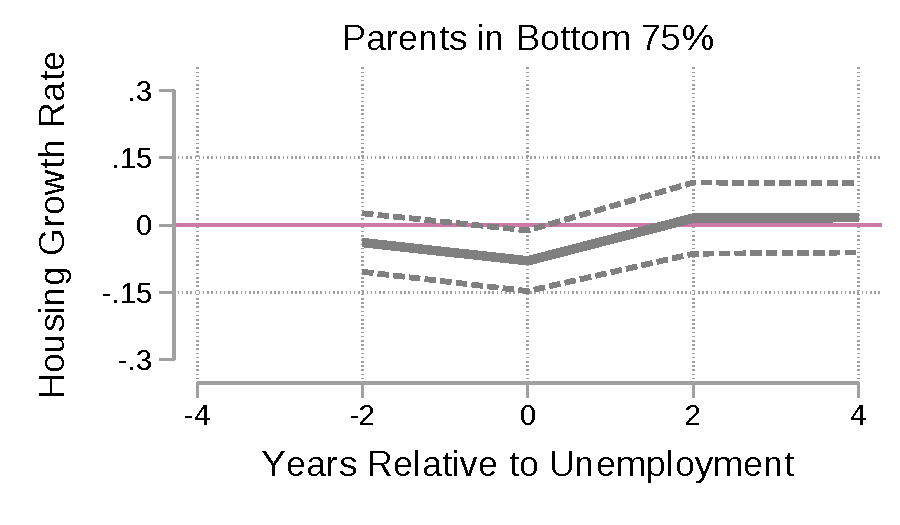
\includegraphics[width=0.5\textwidth]{../tabfig/descr/PSID_housinggrowthpoor_both_controls}%
	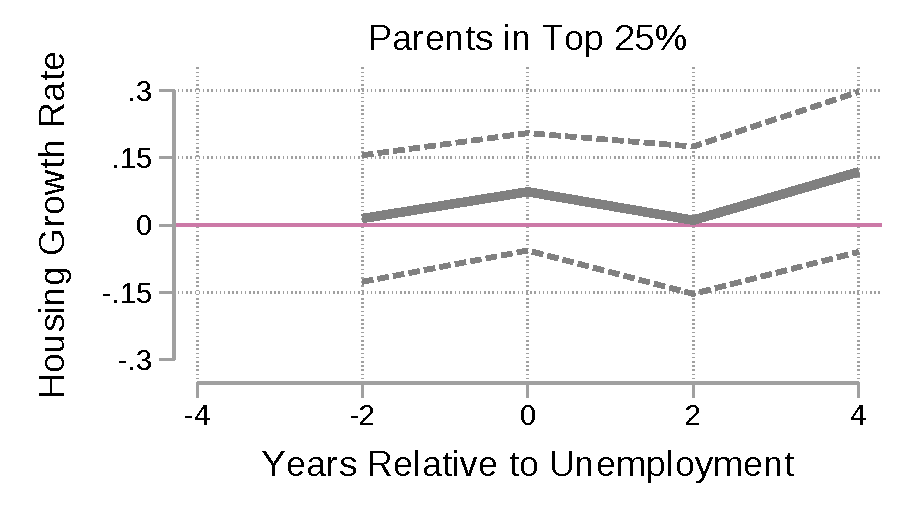
\includegraphics[width=0.5\textwidth]{../tabfig/descr/PSID_housinggrowthrich_both_controls}
	
	{\begin{footnotesize} \textit{Notes:} Solid lines denote means and dashed lines denote the 95\% confidence interval. Sample consists of households aged 25-45 with exactly one observed unemployment spell and without changes in head and/or spouse in the four years before and after unemployment. The reference (omitted) category is four years before unemployment. \end{footnotesize}}
\end{figure}

\section{Supplementary Figures and Tables}
\begin{table}
	\small	
	\caption{Variable Definitions in the PSID}\label{tab:vardef}
	\begin{threeparttable}
	\begin{tabular}{@{}llll@{}}
		\toprule
		Variable& PSID code & Description & Note \\ \midrule
		\textit{Transfer Related} \\ 
		Received Transfer & ER67962 & 2/5years, gift/inherit \$10,000+ & Changing def. \\
		Gave Transfer & RT13V125 & Loans/gifts to child in 2012 & 2013
		prnt/chld file \\ 
		Transfer Amount & RT13V125 & Amount given in 2012 & 2013 prnt/chld file \\
		\textit{Other} \\ 
		Behind Mortgage & ER66062 & Behind on mortgage payments\\
		Income & ER65349 & Total Household Income & \\
		Employment & ER66164 & Working, Unemployed etc. \\
		House Value & ER60031 & Reported Market Value & \\
		Dollars Rent &	ER66090 & Monthly Rent\\
		Family Weight &		ER71570 & Weight of family unit & \\
		\bottomrule
	\end{tabular}
	{\textit{Notes:} This table lilsts the main variables I use from the PSID, as well as their variable code in the 2017 Main family level data set or the 2013 Transfer supplement.}
	\end{threeparttable}
	
\end{table}

\begin{table}
	\centering
	\begin{threeparttable}
		\caption{Housing Choices and Parental Wealth}
		\label{tab:hypo_long}
		\small 
				{
\def\sym#1{\ifmmode^{#1}\else\(^{#1}\)\fi}
\begin{tabular}{l*{5}{c}}
\toprule
                &\multicolumn{1}{c}{(1)}&\multicolumn{1}{c}{(2)}&\multicolumn{1}{c}{(3)}&\multicolumn{1}{c}{(4)}&\multicolumn{1}{c}{(5)}\\
                &\multicolumn{1}{c}{OLS}&\multicolumn{1}{c}{OLS}&\multicolumn{1}{c}{OLS}&\multicolumn{1}{c}{OLS}&\multicolumn{1}{c}{FE}\\
\midrule
\;Par. Wealth   &   -0.007\sym{+}  &   -0.010         &   -0.009\sym{***}&   -0.002         &   -0.007\sym{+}  \\
                &  (0.004)         &  (0.008)         &  (0.002)         &  (0.002)         &  (0.004)         \\
\;Net Worth     &                  &   -0.004         &                  &   -0.004\sym{*}  &    0.006\sym{+}  \\
                &                  &  (0.004)         &                  &  (0.002)         &  (0.003)         \\
\;Income        &                  &    0.002         &                  &   -0.008\sym{+}  &   -0.005         \\
                &                  &  (0.009)         &                  &  (0.004)         &  (0.008)         \\
\;High School=1 &                  &   -0.021         &                  &   -0.002         &    0.003         \\
                &                  &  (0.028)         &                  &  (0.011)         &  (0.013)         \\
\;College=1     &                  &   -0.013         &                  &   -0.011         &    0.037         \\
                &                  &  (0.027)         &                  &  (0.011)         &  (0.027)         \\
\;Married=1     &                  &   -0.022         &                  &   -0.022\sym{*}  &   -0.000         \\
                &                  &  (0.018)         &                  &  (0.010)         &  (0.023)         \\
\;White=1       &                  &    0.030\sym{*}  &                  &   -0.013\sym{*}  &   -0.001         \\
                &                  &  (0.014)         &                  &  (0.007)         &  (0.013)         \\
\;Family Size   &                  &    0.034\sym{+}  &                  &    0.018\sym{*}  &    0.017         \\
                &                  &  (0.018)         &                  &  (0.007)         &  (0.017)         \\
\midrule
N               &      957         &      623         &    5,369         &    4,669         &    4,669         \\
Outcome (mean)  &    0.016         &    0.016         &    0.024         &    0.020         &    0.020         \\
First-Time Buyers Only&        Y         &        Y         &        N         &        N         &        N         \\
Other Controls  &        N         &        Y         &        N         &        Y         &        Y         \\
\bottomrule
\end{tabular}
}

	
	\end{threeparttable}
	{\begin{footnotesize}\begin{flushleft}
		\textit{Notes:} Standard errors in parentheses, clustered at the household level. `Behind' refers to whether the household is behind on a mortgage. Wealth, income, parental wealth, mortgage, family size, and house values are logged. All regressions include year and state fixed effects and control for age and age-squared of both the child and parent. Specifications 1 and 2 use OLS while specifications 3 and 4 use RE and FE, respectively. \textsuperscript{+}$p<0.10$, \textsuperscript{*}$p<0.05$, \textsuperscript{**}$p<0.01$, \textsuperscript{***}$p<0.001$.
		\end{flushleft}\end{footnotesize}}	
\end{table}




\begin{figure}\caption{Calibrated Income Process}\label{fig:calincome}
	\begin{subfigure}{0.49\textwidth}\caption{Deterministic Income Profile $l_a$}\label{fig:y_a}
		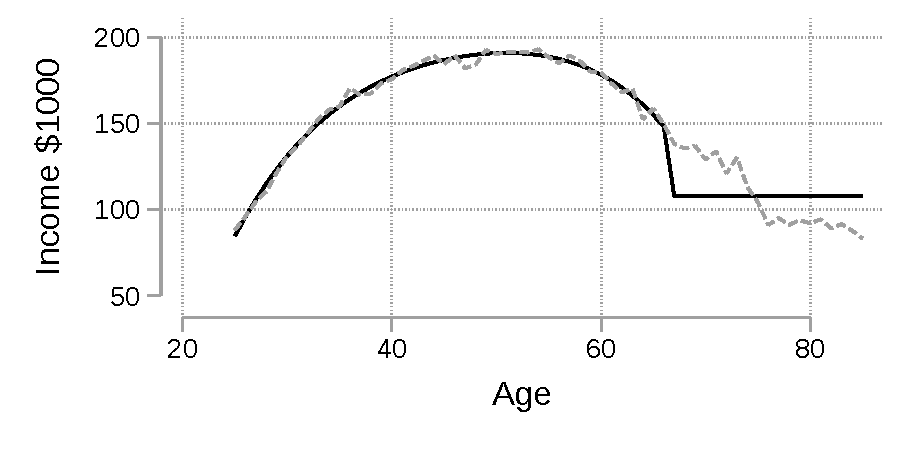
\includegraphics[width=\textwidth]{../tabfig/empirical/lifecycleincome.pdf}%
	\end{subfigure} %
	%
	\begin{subfigure}{0.49\textwidth}\caption{Productivity Shifter $y_{i,a}$}\label{fig:y_ia}
		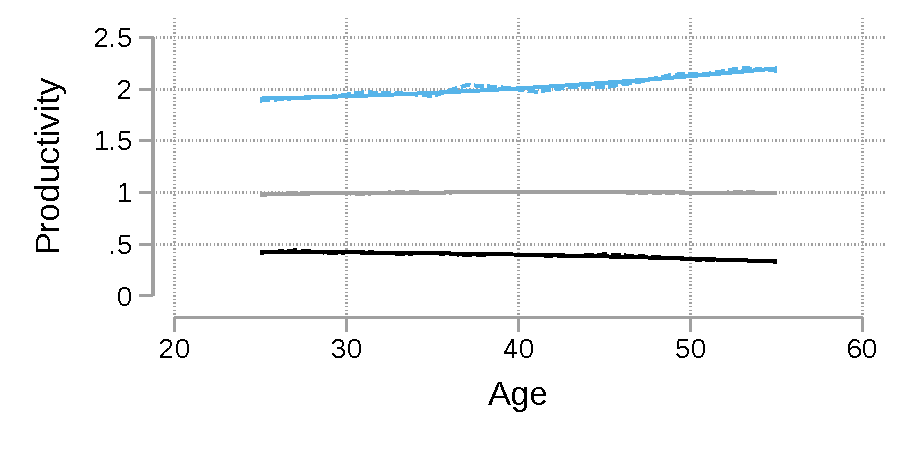
\includegraphics[width=\textwidth]{../tabfig/empirical/lifecycleproductivity_3.pdf}
	\end{subfigure}

	\begin{subfigure}{\textwidth}\caption{Age and State Dependent Productivity Transition Probabilities $\Pi_a(y_{i,a+2}|y_{i,a})$}\label{fig:Piv}
		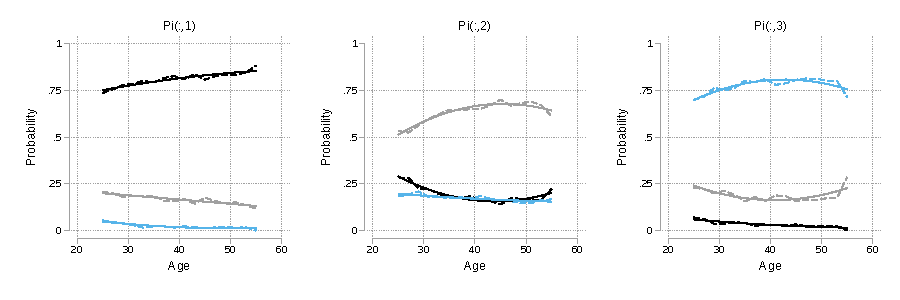
\includegraphics[width=0.99\textwidth]{../tabfig/empirical/Pi_vk_3.pdf} 

		{\begin{footnotesize}\textit{Notes:}
			Dashed lines are the empirical means and solid lines are the fitted polynomials. The top-left panel plots the income level, the top-right panel plots the productivity levels, and the bottom panel plots the transition probabilities (Eq. \ref{eq:wk}). Each line in the bottom panel gives the probability of moving to the bottom tertile (black), middle (gray), and top (blue) income tertiles by the income tertile the child is currently in, by age. \end{footnotesize}\vspace{0.05in}}
	\end{subfigure}
\end{figure}

\begin{figure}\caption{Initial Distribution $F(x_{53},y_{53})$ by wealth $x_{53}$ and productivity $y_{53}$}\label{fig:inidistr}
		
		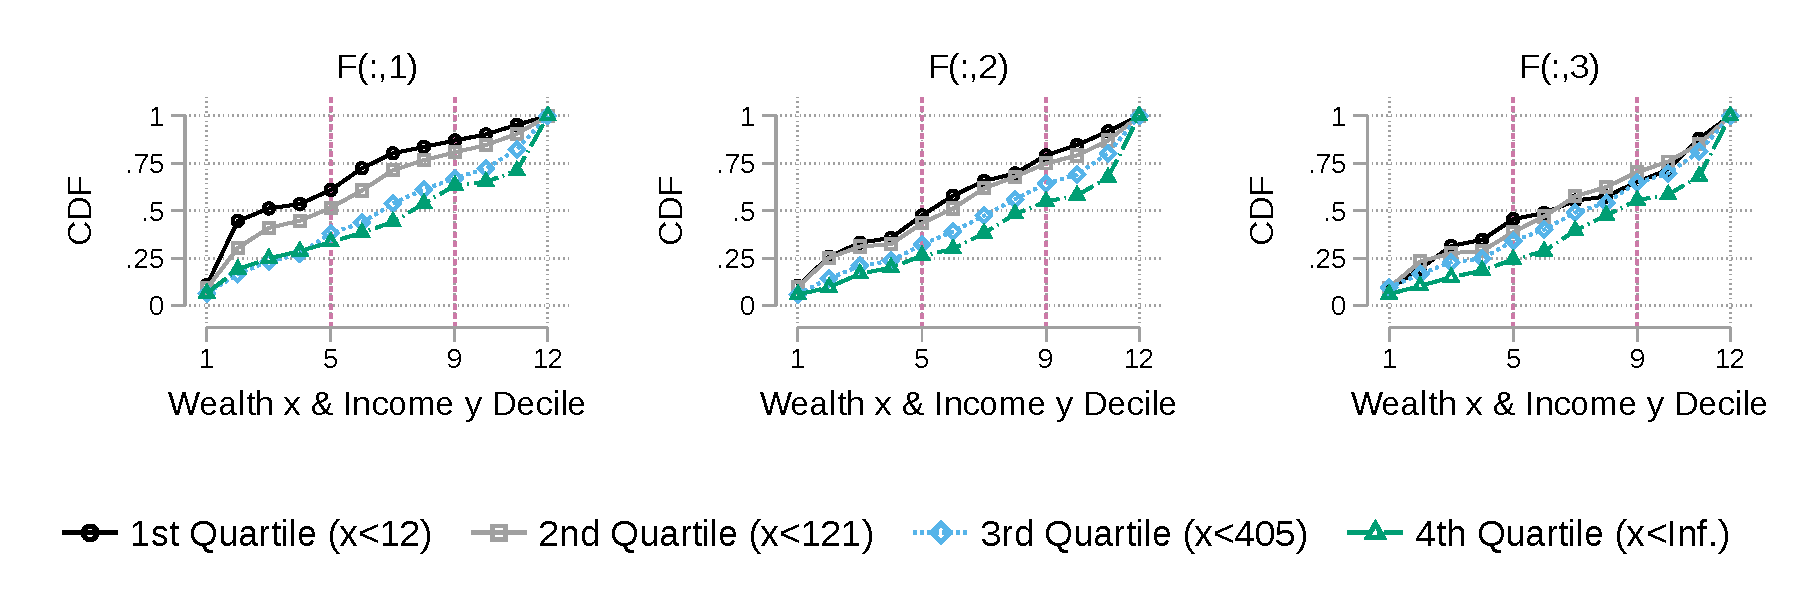
\includegraphics[width=1\textwidth]{../tabfig/empirical/inidistr} 
		{\begin{footnotesize}\textit{Notes:} The vertial lines denote the first, second, and third productivity level for the child. Within each interval each point denotes a wealth quartile. For example, the first point on the black line in the left-most panel gives the probability that a new parent in the first wealth quartile (black lines) and the first income tertile (left panel), has a child in the lowest income tertile and lowest wealth tertile. The second point gives the probability that the child is in the second wealth quartile but first income tertile. \end{footnotesize}}
\end{figure}

\end{document}




